%% Last Update: 29 Oct 2019
%

%% ============================================================================
% فایل  Boostan-LoadBasicPackage یکسری بسته‌های پایه را به استایل اضافه می‌کند. اگر بسته‌ای وجود دارد که در اکثر نوشتارهای خود از آن استفاده می‌کنید، بهتر است آن را در این فایل وارد کنید. 
%% Last Update: 22 Sep 2022
%

%% =========================================================================================================================
%% در مورد تقدم و تاخر وارد کردن بسته ها تنها باید به چند نکته دقت کرد:
%% الف) بسته xepersian حتما حتما باید آخرین بسته ای باشد که فراخوانی می شود، به استثنای بسته  های bidi
%% ب) بسته hyperref جزو آخرین بسته هایی باید باشد که فراخوانی می شود.
%% ج) بسته glossaries حتما باید بعد از hyperref فراخوانی شود. 
%% د) بسته listings باید حتما قبل از  hyperref فراخوانی شود. 

%\usepackage{etex}
%\reserveinserts{28}

% تمام بسته های مورد نیاز برای  کارهای ریاضیاتی به صورت کامل اینجا آورده شده است در صورتی که بخواهید از بسته های دیگر استفاده کنید بهتر است که آن‌ها را به گونه ای انتخاب کنید که با این بسته ها تداخل نداشته باشد. به نظر من استفاده از همین بسته ها کافی است.
% amsthm: It introduces the proof environment and the \theoremstyle command.
% amssymb: It adds new symbols in to be used in math mode.
% amsmath: It contains the advanced math extensions for LaTeX. The complete documentation should be in your LaTeX distribution; the file is called amsdoc, and can be dvi or pdf.

\usepackage{amsthm,amsmath,amssymb}
%\usepackage{thmtools}
%\usepackage{dsfont}
% بسته‌های برای یک سری notation های خاص
\usepackage{wasysym}
%\usepackage{marvosym}

% بسته‌ای برای تنظیم حاشیه و کادر دور فرمول و ... 
%\usepackage{empheq,fancybox}

% بسته biditools امکانات مشابهی و حتی بیشتر از امکاناتی که بسته etoolbox دارد در اختیار شما قرار می‌دهد. بنابراین راه‌حل شما این است که از بسته etoolbox استفاده نکنید و به جای استفاده از دستور \AtBeginEnvironment از دستور \bidi@AtBeginEnvironment استفاده نمایید.
%\usepackage{etoolbox}

% بسته ای بر rotate کردن
\usepackage{rotating}

% بسته‌ای برای فعال‌سازی پارامتر H در وارد کردن شکل. این پارامتر شکل را در همان‌جایی که دقیقا فراخوانی کرده‌ایم، وارد می‌کند.
\usepackage{float}

% برای تنظیم حاشیه صفحات
\usepackage{geometry}

% بسته ای برای تنظیم فونت، اندازه و نحوه نمایش caption
\usepackage{subcaption}

% برای رنگی کردن متن و استفاده از رنگ در متن این دو بسته مورد نیاز است.
\usepackage[usenames,dvipsnames]{xcolor}
\usepackage{eso-pic}
% بسته ای برای وارد کردن Watermarking
%\usepackage{draftwatermark}

%برای قراردادن QR
\usepackage{qrcode}

% It extends the possibility of LaTeX to handle tables, fixing some bugs and adding new features. Using it, you can create very complicated and customized tables. For more information, see the Tables section.
%\usepackage{array}

% بسته ای برای استفاده از اشکال برای آیتم‌ها
\usepackage{pifont}

% بسته ای برای این که در جدول یک متن را در چند سطر بیاوریم. 
\usepackage{multirow}

%
\usepackage{booktabs}
\setlength{\heavyrulewidth}{1.5pt}
\setlength{\abovetopsep}{4pt}

% بسته‌ای برای رسم اشکال و تصاویر با Latex
\usepackage{framed}
\usepackage{tikz}
\usetikzlibrary{calc}

%بسته لازم برای تعریف برخی محیط‌ها به مانند note، refer, point و ...
\RequirePackage[framemethod=TikZ]{mdframed}
%\RequirePackage{tikzpagenodes}

%بسته‌ای برای حل مشکل فونت‌های سری IR
\usepackage[explicit]{titlesec}
%\usepackage{varwidth}

% Line spacing
%To change line spacing in the whole document use the command \linespread covered in Text Formatting.
 %To change line spacing in specific environments use setspace
\usepackage{setspace}

% بسته ای برای وارد کردن الگوریتم در متن
%\usepackage{algorithm}
%\usepackage{algorithmicx}
%\usepackage{algpseudocode}

% در این قالب از بسته graphx برای انجام کارهای گرافیکی استفاده می‌شود. این بسته برای اضافه کردن تصویرها به متن استفاده شده است.
\usepackage{graphicx}

% بسته‌ای است که توسط آن می‌توان شماره صفحه و آخرین صفحه را استخراج نمود. 
%\usepackage{lastpage}
%\usepackage{afterpage}

% بسته‌ای برای قرار گرفتن caption در کنار تصویر در سمت راست تصویر
%\usepackage{sidecap}

% بسته‌ای برای وارد کردن صفحات pdf در متن
\usepackage{pdfpages}

% دوبسته برای اضافه کردن دستورات if و else به برنامه.
\usepackage{xparse}
\usepackage{ifthen}
% بسته‌ای برای رنگ آمیزی جداول
\usepackage{colortbl}

% بسته‌ای برای قراردادن متن در کنار عکس.
\usepackage{wrapfig}
\usepackage{LobsterTwo}
\usepackage{epigraph}

% بسته ای برای هایلایت کردن متن
\usepackage{bidihl}

%برخی بسته‌های مورد نیاز برای استایل pres
\makeatletter
\ifthenelse{\equal{\@docStyle}{Pres}}
{
	\usepackage{sectsty}
	\usepackage{relsize}
}{}
\makeatother

\usepackage{fancyhdr}

% بسته ای برای وارد کردن کدهای برنامه نویسی (MATLAB، JAVA و ...) در متن. بسته listings باید قبل از hyperref باشد و گرنه با خطا مواجه خواهیم شد. برای مطالب بیشتر در مورد نحوه کارکرد این بسته سایت زیر را مشاهده کنید.
% http://www.parsilatex.com/mediawiki/index.php?title=%D8%B1%D8%A7%D9%87%D9%86%D9%85%D8%A7%DB%8C_%D9%88%D8%A7%D8%B1%D8%AF_%DA%A9%D8%B1%D8%AF%D9%86_%DA%A9%D8%AF_%D8%AF%D8%B1_%D9%85%D8%AA%D9%86
\usepackage{listings}

% بسته‌ای برای وارد کردن نمایه ها (index) در متن
\usepackage{makeidx}
\makeindex

% بسته‌ای برای این‌که در هر صفحه شماره پاورقی دوباره از یک شروع شود.
%\usepackage{perpage}

% بسته ای برای رنگی کردن لینک ها و فعال سازی لینک ها در یک نوشتار، بسته hyperref باید جزو آخرین بسته‌هایی باشد که فراخوانی می‌شود. 
\usepackage{hyperref}

% بسته‌ای برای وارد کردن واژه نامه در متن، این بسته باید بعد از hyperref حتما صدا زده شود. 
\usepackage[xindy,acronym,nonumberlist=true]{glossaries}


%زی‌پرشین (به انگلیسی: XePersian) یک بسته حروف‌چینی رایگان و متن‌باز برای نگارش مستندات پارسی/انگلیسی با زی‌لاتک است.
% در واقع، زی‌پرشین، کمک می‌کند تا به آسانی، مستندات را به پارسی، حروف‌چینی کرد. این بسته را وفا خلیقی نوشته است،
% و به طور منظم، آن را بروز‌رسانی کرده و باگ‌های آن را رفع می‌کند.
% نکته مهم این جا است که بسته Xepersian برای پشتیبانی از زبان فارسی آورده شده است، و 
% می بایست آخرین بسته ای باشد که شما وارد می کنید، دقت کنید: آخرین بسته 
\usepackage[extrafootnotefeatures]{xepersian}


% یکسری فر امین اصلی نیز در فایل Boostan-BasicCommand ارایه شده است. 
%% توسط دستور \myData می توانید تاریخ و ساعت را وارد متن خود کنید. 
\newcommand{\myData}{
	\newcount \hour
	\newcount \min
	\newcommand*{\timeoftoday}{%
		\hour\time\divide\hour 60 ساعت \the\hour{}
		\min\time\multiply\hour 60 \advance\min-\hour
		\ifnum\min=0
		\else
		و
		\the\min{} دقیقه
		\fi}
	\today{} در \timeoftoday
} %M



%%% =========================================================================================================================

%%% اضافه کردن نماد استقلال به علایم ریاضی
\newcommand{\Perp}{\perp \! \! \! \perp}
\newcommand{\independent}{\protect\mathpalette{\protect\independenT}{\perp}} \def\independenT#1#2{\mathrel{\rlap{$#1#2$}\mkern2mu{#1#2}}}

%%% این دستور به این خاطر تعریف می‌شود، که اگر بخواهیم مثلا یک کلمه در واژه نامه را Index‌کنیم، مثلا بنویسیم، ‎\index{\glspl{Water}‎}‎، این دستور index درست عمل نمی‌کند. نویسنده بسته glossaries در این باره این طور گفته است.
%%%If you inspect the .idx file you will see that it contains the following:
%%%\indexentry{\glsentryplural{StrictlyStable}|hyperpage}{1}
%%%\index doesn't expand its argument when writing to the .idx file and since xindy doesn't understand (La)TeX commands the index won't be correctly sorted. This is a feature of \index and is not connected with glossaries.
%%%You could try something like
%%%\expandafter\index\expandafter{\glsentryplural{StrictlyStable}}
%%% توسط دستور تعیین شده می‌توان این مشکل را حل کرد. دقت کنید که این دستور می‌بایست حتما برای واژه‌نامه ها فقط تعریف شود.

%\let\oldindex\index
%\renewcommand{\index}[1]{
%\ifthenelse{\equal{\glsentrytype{#1}}{english}}
	%{\expandafter\oldindex\expandafter{\glsentrytext{#1}}}
	%{ \ifthenelse{\equal{\glsentrytype{#1}}{acronym}}
		%{\expandafter\oldindex\expandafter{\glsentrytext{#1}}}
		%{\oldindex{#1}}
	%}
%}

%%% گاهی اوقات مطلبی را در یک بخش، فصل و ... می‌نویسیم، وقتی این مطلب را در متن ارجاع می دهیم، مثلا می نویسیم بخش ‎\ref{seclabel}‎، اما ممکن است به هر علتی مطلب ما از بخش به فصل و یا به یک زیربخش تنزل پیدا کند.
%%% بدین‌منظور به جای دستور ref از autoref استفاده می‌کنیم. در این صورت خود latex می‌فهمد که این مطالب در ‎چه قسمتی است و خودش کلمه فصل، بخش و یا ... را قبل از شماره آن اضافه می‌کند. دستورات زیر می‌گوید در هر یک 
%%% از سطوح متن چه کلمه‌ای‌ قرار گیرد. 
\def\sectionautorefname{بخش}
\def\subsectionautorefname{زیربخش}
\def\subsubsectionautorefname{زیربخش}


% حل شدن مشکل part
%%%% تعریف یکسری دستور به منظور حل مشکل قرار دادن part در متن و آمدن آن در فهرست مطالب. 
\makeatletter
\renewcommand*\l@part[2]{
	\ifnum \c@tocdepth >-2\relax
	\addpenalty{-\@highpenalty}
	\addvspace{2.25em \@plus\p@}
	\setlength\@tempdima{3em}
	\begingroup
	\parindent \z@ \if@RTL\leftskip\else\rightskip\fi \@pnumwidth
	\parfillskip -\@pnumwidth
	{\leavevmode
		\large \bfseries\textcolor{blue}{بخش} #1
		\hfil \hb@xt@\@pnumwidth{\hss #2}}\par
	\nobreak
	\global\@nobreaktrue
	\everypar{\global\@nobreakfalse\everypar{}}
	\endgroup
	\fi}
\makeatother

\makeatletter
\def\@chapter[#1]#2{\ifnum \c@secnumdepth >\m@ne
	\if@mainmatter
	\refstepcounter{chapter}%
	\typeout{\@chapapp\space\thechapter.}%
	\addcontentsline{toc}{chapter}%
	{\@chapapp~\protect\numberline{\arabic{chapter}}~~~ #1}%
	\else
	\addcontentsline{toc}{chapter}{#1}%
	\fi
	\else
	\addcontentsline{toc}{chapter}{#1}%
	\fi
	\chaptermark{#1}%
	%\addtocontents{lof}{\protect\addvspace{10\p@}}%
	%\addtocontents{lot}{\protect\addvspace{10\p@}}%
	\if@twocolumn
	\@topnewpage[\@makechapterhead{#2}]%
	\else
	\@makechapterhead{#2}%
	\@afterheading
	\fi}
%\renewcommand*\l@section{\@dottedtocline{1}{4.5em}{2.3em}}
%\renewcommand*\l@subsection{\@dottedtocline{2}{6.5em}{3.2em}} 
\makeatother

%%% این دستور به این خاطر تعریف می‌شود، که اگر بخواهیم مثلا یک کلمه در واژه نامه را Index‌کنیم، مثلا بنویسیم، ‎\index{\glspl{Water}‎}‎، این دستور index درست عمل نمی‌کند. نویسنده بسته glossaries در این باره این طور گفته است.
%%%If you inspect the .idx file you will see that it contains the following:
%%%\indexentry{\glsentryplural{StrictlyStable}|hyperpage}{1}
%%%\index doesn't expand its argument when writing to the .idx file and since xindy doesn't understand (La)TeX commands the index won't be correctly sorted. This is a feature of \index and is not connected with glossaries.
%%%You could try something like
%%%\expandafter\index\expandafter{\glsentryplural{StrictlyStable}}
%%% توسط دستور تعیین شده می‌توان این مشکل را حل کرد. دقت کنید که این دستور می‌بایست حتما برای واژه‌نامه ها فقط تعریف شود. 
\newcommand{\indexglspl}[1]{\expandafter\index\expandafter{\glsentryplural{#1}}}
\newcommand{\indexgls}[1]{\expandafter\index\expandafter{\glsentryname{#1}}}


% تنظیمات مربوط به بسته‌ها
%% Last Update: 28 Jul 2019
%

%% ==========================================================================
% تنظیمات بسته geometry که مربوط به حاشیه صفحه می‌شود. 
\makeatletter
\ifthenelse{\equal{\@docStyle}{Report}}{\geometry{a4paper,top=2.4cm, bottom=2.6cm, left=2cm, right=2.1cm}}{
  \ifthenelse{\equal{\@docStyle}{Pres}}  {\geometry{a4paper,landscape,top=1.8cm,bottom=.7cm,left=1cm,right=1cm,includefoot,verbose,nohead,footskip=.5cm,bmargin=8mm}}{
    \geometry{a4paper,top=2.4cm, bottom=2.6cm, left=2cm, right=2.1cm} %Default
  }
}
\makeatother
% در Latex انواع مختلفی از اندازه‌ها برای ابعاد کاغذ وجود دارد. گرچه شما می‌توانید به دلخواه ابعاد مختلفی به کاغذ بدهید. 
%a0paper, a1paper, a2paper, a3paper, a4paper, a5paper, a6paper,b0paper, b1paper, b2paper, b3paper, b4paper, b5paper, b6paper, c0paper, c1paper, c2paper, c3paper, c4paper, c5paper, c6paper, b0j, b1j, b2j, b3j, b4j, b5j, b6j, ansiapaper, ansibpaper, ansicpaper, ansidpaper, ansiepaper, letterpaper, executivepaper, legalpaper


%% ==========================================================================
% تنظیمات listing مربوط به وارد کردن کد در متن
%% Date: 24 Jul 2019
%

%%% =========================================================================================================================
%%==================== تنظیمات listing
%%  در این قسمت تمام ابزارهای مورد نیاز در نوشتن برنامه ها اورده شده  است. با استفاده از این ابزارهای می‌توان برنامه های مورد نیاز را در مستند جای داد.
%% مطالب بیشتر در مورد وارد کردن کد در متن را در صفحه زیر مطالعه کنید.
%%%http://www.parsilatex.com/mediawiki/index.php?title=%D8%B1%D8%A7%D9%87%D9%86%D9%85%D8%A7%DB%8C_%D9%88%D8%A7%D8%B1%D8%AF_%DA%A9%D8%B1%D8%AF%D9%86_%DA%A9%D8%AF_%D8%AF%D8%B1_%D9%85%D8%AA%D9%86

\lstset{% general command to set parameter(s)
	% زبان برنامه نویسی که به طور پیش فرض انتخاب می شود.
	%language=Java,
	% رنگ پیش فرض برای پیش زمینه
	%backgroundcolor=\color{gray!10},
	%% میزان طول محیط listings را مشخص می کند، به صورت پیش فرض \textwidth است. 
	%linewidth=\textwidth ,
	%% نوع قالب دور محیط listings را تعیین می کند. 
	frameround=fttt,
	frame=single,
	aboveskip=5mm,
	belowskip=4mm,
	%% is selected at the beginning of each listing. You could use \footnotesize,
	%% \small, \itshape, \ttfamily, or something like that. The last token of
	%% basic style must not read any following characters.
	basicstyle=\setLTR\ttfamily, % print whole listing small
	%%   با این دستور استایل keyword ها را مشخص می کنیم. مثلا در این حالت گفته ایم که keyword ها را با رنگ آبی مشخص کند، و آن ها را bold‌کند. دقت کنید که keyword های زبان‌هایی که این بسته پشتیبانی می‌کند، 
	%% در این بسته تعریف شده است. مثلا در JAVA کلمه main به صورت پیش فرض تعریف شده است و در صورت وجود آن در کد شما آن را Latex آبی رنگ می‌کند. 
	keywordstyle=\color{blue}\bfseries,
	% underlined bold black keywords
	%identifierstyle=, % nothing happens
	%framexleftmargin=5mm, frame=shadowbox, rulesepcolor=\color{red}
	%% استایل String را در متن مشخص می کند. مثلا در این جا گفته شده است که رشته ها را با رنگ قرمز و به صورت ایتالیک نمایش بده.
	stringstyle=\ttfamily\color{red}, % typewriter type for strings
	%% نحوه استایل comment را مشخص می کند. دقت کنید که رنگ انتخاب شده نوعی رنگ سبز است، برای این که این رنگ شناخته شود می بایست دو بسته color و xcolor به صورتی که فراخوانی شده است، فراخوانی شود. 
	commentstyle=\color{Green},
	lineskip = 1mm,
	%% سه دستور بعدی نحوه نمایش شماره خطوط را مشخص می کند. 
	numberstyle=\footnotesize, 
	%% تعیین فاصله بین شماره خطوط و محیط listings
	numbersep=10pt,
	%% محل قرارگیری شماره خطوط
	numbers=left,
	xleftmargin=1pt,aboveskip=7mm,belowskip=6mm,
	%% تعیین محل قرارگیری caption محیط. بطور پیش فرض در بالای محیط است که به پایین محیط تغییر داده شده است. 
	%captionpos=b, 
	%% توسط breakline می توانید خاصیت شکسته شدن خطوط بلند را در محیط listings فعال و یا غیرفعال کنید.
	%% activates or deactivates automatic line breaking of long lines.
	breaklines=true,
	%% باعث می شود که فاصله های بین رشته های نمایان شود.
	%% lets blank spaces in strings appear  or as blank spaces
	%showstringspaces=true
	captiondirection=RTL
}%

\lstdefinestyle{customc}{
	belowcaptionskip=1\baselineskip,
	breaklines=true,
	frame=L,
	backgroundcolor=\color{white}
	xleftmargin=\parindent,
	language=C,
	showstringspaces=false,
	basicstyle=\setLTR\small\ttfamily,
	keywordstyle=\bfseries\color{green!40!black},
	commentstyle=\itshape\color{purple!40!black},
	stringstyle=\color{orange},
	numbers=none
}

\renewcommand{\lstlistingname}{\rl{کد}}

% البته شما می توانید این موارد پیش فرض را به ازای هر کد تغییر دهید. به عنوان مثال، ما یک کد در پوشه Code در شاخه فعلی قرار دادیم، می خواهیم آن را وارد متن کنیم، کافی است که خطوط زیر را در محل مناسبی که می خواهیم کد را قرار دهیم وارد کنیم. در این مثال یک فایل کد JAVA به نام myCode.java را می خواهیم وارد کنیم. 
%\begin{latin}
%\lstinputlisting[breaklines=true,numbers=left,language=Java, basicstyle=\ttfamily, numberstyle=\footnotesize, numbersep=10pt, captionpos=b, frame=single, breakatwhitespace=false]{Code/myCode.java}
%\end{latin}



%%% =========================================================================================================================
%تعریف و تکمیل Syntaxhighlight برای برخی از زبان‌های برنامه‌نویسی. 

%% ASN.1
\lstdefinelanguage[]{asn.1}%
{keywords=%
	{DEFINITIONS,SEQUENCE,OCTET,INTEGER,BEGIN,END,OPTIONAL,STRING,ENUMERATED,CHOICE,BOOLEAN},
	sensitive=true,
	morestring=[b]",
	morestring=[s]{>}{<},
	morecomment=[l]{--},
	morecomment=[s]{<?}{?>},
	stringstyle=\color{black},
	identifierstyle=\color{Blue},
	keywordstyle=\color{cyan},
	morekeywords={xmlns,version,type}% list your attributes here
	emph=[2]%
	{%
		DEFAULT,NULL,
	},
	emphstyle=[2]{\color{Red}},
	%
	emph=[3]% Variable Types
	{% 
		SIZE,
	},
	emphstyle=[3]{\color{Plum}},
}[keywords]%


%% XML
\lstdefinelanguage{XML}
{
  morestring=[b]",
  morestring=[s]{>}{<},
  morecomment=[s]{<?}{?>},
  stringstyle=\color{black},
  identifierstyle=\color{Blue},
  keywordstyle=\color{cyan},
  columns=fullflexible,
  showstringspaces=false,
  morekeywords={xmlns,version,type}% list your attributes here
}%


%% JSON
\colorlet{numb}{magenta!60!black}
\lstdefinelanguage{JSON}{
    stepnumber=1,
    numbersep=8pt,
    showstringspaces=false,
    breaklines=true,
    string=[s]{"}{"},
    comment=[l]{:\ "},
    morecomment=[l]{:"},
literate=
        *{0}{{{\color{numb}0}}}{1}
         {1}{{{\color{numb}1}}}{1}
         {2}{{{\color{numb}2}}}{1}
         {3}{{{\color{numb}3}}}{1}
         {4}{{{\color{numb}4}}}{1}
         {5}{{{\color{numb}5}}}{1}
         {6}{{{\color{numb}6}}}{1}
         {7}{{{\color{numb}7}}}{1}
         {8}{{{\color{numb}8}}}{1}
         {9}{{{\color{numb}9}}}{1}
}%


%% INI
\lstdefinelanguage{INI}
{
    morecomment=[s][\color{Orchid}\bfseries]{[}{]},
    morecomment=[l]{\#},
    morecomment=[l]{;},
    commentstyle=\color{gray}\ttfamily,
    morekeywords={},
    otherkeywords={=,:},
    keywordstyle={\color{Green}\bfseries}
}%


%% QT
\lstdefinelanguage{QT}
{
    language=C++,
    keywordstyle={\color{blue}\bfseries},
    keywordstyle=[2]{\color{Plum}\bfseries},
    keywordstyle=[3]\color{Orange},
    keywords=[2]{uint64_t,uint32_t,uint16_t,uint8_t,QByteArray,QObject,QString,QTimer,QSqlDatabase,QSqlQuery,QProcess,QSettings,QFileInfo,QJsonDocument,QStateMachine,QTextCodec,QJsonObject,QRegularExpression,QDomDocument,QXmlStreamReader,QRegExp,QHostAddress,QTextCodec,QMessageBox,QFile,QMainWindow,QDebug,QTime,QThreadPool},
    keywords=[3]{nullptr}
}%


\lstdefinelanguage{Kotlin}{
  comment=[l]{//},
  commentstyle={\color{gray}\ttfamily},
  emph={filter, first, firstOrNull, forEach, lazy, map, mapNotNull, println},
  emphstyle={\color{OrangeRed}},
  identifierstyle=\color{black},
  keywords={!in, !is, abstract, actual, annotation, as, as?, break, by, catch, class, companion, const, constructor, continue, crossinline, data, delegate, do, dynamic, else, enum, expect, external, false, field, file, final, finally, for, fun, get, if, import, in, infix, init, inline, inner, interface, internal, is, lateinit, noinline, null, object, open, operator, out, override, package, param, private, property, protected, public, receiveris, reified, return, return@, sealed, set, setparam, super, suspend, tailrec, this, throw, true, try, typealias, typeof, val, var, vararg, when, where, while},
  keywordstyle={\color{NavyBlue}\bfseries},
  morecomment=[s]{/*}{*/},
  morestring=[b]",
  morestring=[s]{"""*}{*"""},
  ndkeywords={@Deprecated, @JvmField, @JvmName, @JvmOverloads, @JvmStatic, @JvmSynthetic, Array, Byte, Double, Float, Int, Integer, Iterable, Long, Runnable, Short, String, Any, Unit, Nothing},
  ndkeywordstyle={\color{BurntOrange}\bfseries},
  sensitive=true,
  stringstyle={\color{ForestGreen}\ttfamily},
}



%% ===========================================================================
%تنظیمات hyperref

% برای وارد کردن کلمه (بخش) در فهرست مطالب بسته hyperref برای حالت فارسی یک مشکل دارد. بدین منظور این 
% مشکل را به صورت دستی حل شده است. برای این که رنگ keywordstyle که تعیین کننده رنگ کل قسمت فهرست مطالب
% نیز هست یکسان در آید یک پارامتر رنگ برای keywordstyle این جا تعریف می‌کنیم، و سپس از آن هم در تنظمیات hypperref 
% و هم در اون کدهایی که به صورت دستی وارد شده است، استفاده می‌شود.  مطالب بیشتر در مورد این بسته را در سایت زیر مطالعه کنید.
% http://en.wikibooks.org/wiki/LaTeX/Hyperlinks

% در این قسمت تنظیمات بسته hyperref را قرار می دهیم.
% این تنظیمات شامل موارد زیر است:
\hypersetup{
	pdfmenubar=false,			% show or hide Acrobat’s menu
	pdftoolbar=true,			%show or hide Acrobat’s toolbar
%% موقعی که فایل پی دی اف خروجی را باز می کنید صفحه به صورت عریض و بزرگ باز می شود.
	pdfstartview=FitH, 
	%% مواردی که برای فعال سازی این که شماره اشکال را به صورت ارجاعی نشان دهد
	%hyperfigures=true,
	%% به جای استفاده از مربع قرمز دور موارد ارجاعی از لینک های رنگی استفاده کند.
	colorlinks=true, 
	%% رنگ برخی از لینک ها در زیر تعریف شده است. 
	linkcolor=blue, 
	anchorcolor=green, 
	citecolor=magenta, 
	urlcolor=cyan, 
	filecolor=magenta, 
	bookmarkstype=toc,
	unicode = true			%allows to use characters of non-Latin based languages in Acrobat’s bookmarks
	%bookmarksopen = true,
	%bookmarksopenlevel = 1
	%%% اگر این option را true‌ بکنیم، آن‌گاه در کنار bookmark شماره فصل و بخش و زیربخش نیز می آید. مثلا می‌نویسد: ۱.۲ طراحی شبکه
	%bookmarksnumbered = true,
	%hidelinks			%hide links (removing color and border)
} % M


%%% گاهی اوقات مطلبی را در یک بخش، فصل و ... می‌نویسیم، وقتی این مطلب را در متن ارجاع می دهیم، مثلا می نویسیم بخش ‎\ref{seclabel}‎، اما ممکن است به هر علتی مطلب ما از بخش به فصل و یا به یک زیربخش تنزل پیدا کند.بدین‌منظور به جای دستور ref از autoref استفاده می‌کنیم. در این صورت خود latex می‌فهمد که این مطالب در ‎چه قسمتی است و خودش کلمه فصل، بخش و یا ... را قبل از شماره آن اضافه می‌کند. دستورات زیر می‌گوید در هر یک  از سطوح متن چه کلمه‌ای‌ قرار گیرد. لازم به ذکر است که برای این کار به بسته hyperref نیاز است. 
\def\partname{پاره}
\renewcommand{\partautorefname}{پاره}
\def\sectionautorefname{بخش}
\def\subsectionautorefname{زیربخش}
\def\subsubsectionautorefname{زیربخش}
\def\equationautorefname{رابطه}
\def\figureautorefname{شکل}
\def\tableautorefname{جدول}
\def\lemmaautorefname{لم}


%% ====================================================================
%% تنظیمات tikz
%% لازم به ذکر است که کتابخانه های بسته tikz به صورت پیش فرض فعال نشده است، و کاربر به دلخواه خود اگر به مراتب به آن نیاز دارد باید آن را فعال کند. 
%\usetikzlibrary{mindmap,backgrounds,shadows,trees,arrows,shapes,positioning,shadings}
\usetikzlibrary{calc}


%% ====================================================================
%% تنظیمات algorithm و algorithmic
%\floatname{algorithm}{الگوریتم}


%% =====================================================================
%% تنظیمات graphicx
% برای اضافه کردن تصاویر به متن این امکان وجود دارد که تصاویر را در پوشه‌های متفاوت قرار داد. با این کار از زیاد شدن پرونده‌ها در مسیر مستند جلوگیری می شود. علاوه بر این دسته‌ای از تصاویر وجود دارد که بین همه مستندها مشترک است
% برای نمونه نماد پژوهشکده که بین همه مشترک است.  از این رو تعداد مسیر به عنوان مسیرهای پیش فرض برای جستجوی تصاویر تعیین شده است.
%\graphicspath{{../../Pic/}{./Pic/}}


%% =======================================================================
%% تنظیمات مربوط به ایجاد watermarking

%% زاویه متن Watermark
\SetWatermarkAngle{45}
%% اندازه watermark
\SetWatermarkScale{1.5}

\let\oldSetWatermarkText\SetWatermarkText
%% اگر بخواهید watermark شما یک رنگ دیگر داشته باشد، این دو خط را فعال کنید و رنگ مورد نظر خود را انتخاب کنید
%\definecolor{orange}{RGB}{229,252,219} 
%\renewcommand{\SetWatermarkText}[1]{\oldSetWatermarkText{\textcolor{orange}{#1}}}

\DeclareDocumentCommand{\SetWatermarkText}{m g}{
	\oldSetWatermarkText{#1}
	\IfValueTF{#2}{
		\SetWatermarkLightness{#2}
	}{%%
		\SetWatermarkLightness{.94}
	}%%
}%


%% =========================================================================
% تنظیم فونت. 
%برای دانستن اطلاعات بیشتر در مورد تنظیم فونت به لینک زیر مراجعه کنید.
%http://www.parsilatex.com/mediawiki/index.php?title=%D9%81%D9%88%D9%86%D8%AA_%D8%AF%D8%B1_xepersian
% دقت شود که در این استایل از فونت های زیر استفاده می‌شود، بدین‌سان لازم است فونت هایی که فعال هستند (comment نیستند) توسط کاربر در سیستم عامل نصب شود.
%سعی شده است از فونت های استاندارد IR‌ که حاصل کار شورای عالی اطلاع رسانی هست، استفاده شود، کاربران می‌توانند فونت های یاد شده را از لینک زیر دانلود کنند.
% http://www.scict.ir/portal/Home/Default.aspx?CategoryID=b50ee619-ce53-4c25-bf53-b0f0332c1777

% تعریف یک دستور به عنوان فونت پیش فرض
\makeatletter
\newcommand{\defaultFont}{
% با دستور زیر می توانید فونتی مخصوص عبارات فارسی تعیین کنید:
	\ifthenelse{\equal{\@docStyle}{Report}} {\settextfont[Scale=1.25]{IRNazanin}}{
	\ifthenelse{\equal{\@docStyle}{Pres}}   {\settextfont[Scale=1.4]{IRNazanin}}{
	\ifthenelse{\equal{\@docStyle}{Letter}}{\settextfont[Scale=1.25]{IRNazanin}}{}}
	}
% شما با دستور زیر بعد از فراخوانی بسته xepersian می توانید فونت انگلیسی را تعیین کنید
% دقت کنید که عبارات انگلیسی شما باید در دستور \lr{} قرار گیرد تا xepersian بتواند بفمهد که این عبارات انگلیسی است
	\ifthenelse{\equal{\@docStyle}{Report}} {\setlatintextfont[Scale=1.1]{Linux Libertine}}{
	\ifthenelse{\equal{\@docStyle}{Pres}}   {\setlatintextfont[Scale=1.2]{Linux Libertine}}{
	\ifthenelse{\equal{\@docStyle}{Letter}}{\setlatintextfont[Scale=1.1]{Linux Libertine}}{}}
	}
% تعریف برای فونت اعداد و ارقام
	%\setdigitfont[Scale=1.1]{XB Zar}
} % M
\makeatother

\defaultFont

%%  با استفاده از این دستور می‌توان فونت و فارسی و یا انگلیسی بودن اعداد در فرمول‌ها را به حالت اولیه (یعنی پیش‌فرض لاتک) برگرداند.
\DefaultMathsDigits

%% نحوه تغییر اندازه فونت عبارات ریاضی و فرمول‌ها. این کار توسط دستور زیر انجام می‌شود. 
%%\DeclareMathSizes{textsize}{mathsize}{scriptsize}{scriptscriptsize}
%% گزینه اول: این برای چه دسته فونتی است. پیش فرض استایل ما فونت 10pt است. 
%% گزینه دوم: اندازه فونت توابع و موجودات ریاضی درون متن.
%% گزینه سوم: برای اسکریپت ها، اندازه زیرنویس و بالانویس.
%% گزینه چهارم: برای زیرنویس زیرنویس.

%% در دستورات زیر ما برای سه حالت، اندازه‌های مورد نظر را تعریف کرده ایم. 
%%\DeclareMathSizes{10}{11}{9}{8}   % For size 10 text
%%\DeclareMathSizes{11}{12}{11}{10}   % For size 11 text
%%\DeclareMathSizes{12}{13}{12}{11}  % For size 12 text


% فایل  Environments  در برگیرنده تعریف یکسری محیط نوین است. 
%% Data:  2015-10-03
%% تعریف برخی نمادهای item و شماره گذاری برای استفاده
\newcommand{\idx}[1]{\index{#1}#1}
%% می تواند برای ارایه نکات در محیط itemize به کار رود، روند این کار به این صورت است،  (شکل یک تیر)
\newcommand{\arcm}{\item[\Large\color{red}\ding{247}]}
\newcommand{\arcmO}{\noindent\textcolor{red}{\Large\ding{247}}\;}
%% این شکل می‌تواند برای بیان مزایای یک قضیه بکار رود (شکل تیک)
\newcommand{\tick}{\item[\large\color{green}\ding{52}]}
\newcommand{\tickO}{\noindent\textcolor{green}{\Large\ding{52}}\;}
%% برای  بیان معایب و یا نکات منفی (شکل یک ضربدر)
\newcommand{\X}{\item[\Large\color{red}\ding{56}]}
\newcommand{\XO}{\noindent\textcolor{red}{\LARGE\ding{56}}\;}
%% بیان موارد یک قضیه (شکل یک دست)
\newcommand{\hand}{\item[\Large\color{blue}\ding{45}]}
\newcommand{\handO}{\noindent\textcolor{blue}{\LARGE\ding{45}}\;}
%% برای مواردی که: این موارد شامل .... می شود، توسط عناصر زیر مشخص می شود (شکل یک درخت)
%% برای نوشتن  پارامتر‌ها، 
\newcommand{\tree}{\item[\Large\color{ForestGreen}\ding{171}]}
\newcommand{\treeO}{\noindent\textcolor{ForestGreen}{\Large\ding{171}}\;}
%% برای این که چند مورد را تعریف کنیم (علامت دست که دو گرفته)
\newcommand{\two}{\item[\LARGE\color{blue}\ding{44}]}
\newcommand{\twoO}{\noindent\textcolor{blue}{\LARGE\ding{44}}\;}
%% (شکل یک قیچی)
\newcommand{\sci}{\item[\footnotesize\color{OrangeRed}\ding{108}]}
\newcommand{\sciO}{\noindent\textcolor{OrangeRed}{\footnotesize\ding{108}}\;}

\newcommand{\starE}{\item[\Large\color{Plum}\ding{97}]}
\newcommand{\starEO}{\noindent\textcolor{Plum}{\Large\ding{97}}\;}
%% برای حالت‌هایی که فرضیات داریم. 
\newcommand{\music}{\item[\Large\color{Green}\ding{161}]}
\newcommand{\musicO}{\noindent\textcolor{Green}{\Large\ding{161}}\;}

\newcommand{\gol}{\item[\Huge\color{RubineRed}\ding{96}]}
\newcommand{\golO}{\noindent\textcolor{RubineRed}{\Huge\ding{96}}\;}

%%% =========================================================================================================
%% با دستور newtheoremstyle شما می توانید یک استایل جدید برای محیط هایی چون plain، definition‌ و ... تعریف کنید. شکل کلی این دستور به صورت زیر است.

%%\newtheoremstyle{stylename}% name of the style to be used
%%  {spaceabove}% measure of space to leave above the theorem. E.g.: 3pt
%%  {spacebelow}% measure of space to leave below the theorem. E.g.: 3pt
%%  {bodyfont}% name of font to use in the body of the theorem
%%  {indent}% measure of space to indent
%%  {headfont}% name of head font
%%  {headpunctuation}% punctuation between head and body
%%  {headspace}% space after theorem head; " " = normal interword space
%%  {headspec}% Manually specify head
% % تعریف محیط‌های گوناگون مانند محیط برای قضیه و ... 
%% theoremstyle = > plain, definition, remark 


\setlength{\topsep}{0pt}

%% با دستور newtheorem یک نوع از استایلی که در بالای آن تعریف شده است ایجاد می کنیم. 
\theoremstyle{plain}
\newtheorem{theorem}{قضیه}[chapter]
\newtheorem{principle}{اصل}
\newtheorem{proposition}{گزاره}
\newtheorem{lemma}{لم}[chapter]
\theoremstyle{definition}
\newtheorem{definition}{تعریف}[chapter]
\newtheorem{example}{مثال}
\newtheorem{prob}{سوال}
\theoremstyle{remark}
\newtheorem{corollary}{نتیجه}[chapter]
\newtheorem{property}{نکته}
\newtheorem{remark}{ملاحظه}

%\declaretheoremstyle[headfont=\bfseries, notefont=\bfseries , postheadspace=\newline]{mystyle}
%\declaretheorem[style=mystyle,name=تعریف]{definition}
%
%\let\olddefnition\definition
%\let\oldenddefnition\enddefinition
%\renewenvironment{definition}{
%\olddefnition
%}{
%\begin{latin}
%\vskip -3mm
%\ding{36} ------------------
%\end{latin}
%\oldenddefnition
%}

%% در این جا محیط proof را باز تعریف می‌کنیم.
\let\oldproof\proof
\let\oldendproof\endproof
\def\proof{\par\noindent\textcolor{red}{\textbf{اثبات.}} }
\def\endproof{\vskip -5mm\hfill$\blacksquare$\oldendproof}

%% تعریف یک محیط برای  اثبات لم ها. در این محیط بر خلاف محیط proof ساده، یک مربع توخالی می‌گذارد. 
\def\lemmaproof{\par\noindent\textcolor{ForestGreen}{\textbf{اثبات لم.}} }
\def\endlemmaproof{\vskip -5mm\hfill$\square$\oldendproof}

%%% =========================================================================================================

%% %% در ادامه یکسری محیط جالب به صورت کادر رنگی برای استفاده های مختلف تعریف می شود. 
 
\makeatletter
\newdimen\errorsize \errorsize=0.2pt
% Frame with a label at top
\newcommand{\LabFrame}[2]{
	\baselineskip=.4cm
	\fboxrule=\FrameRule
	\fboxsep=-\errorsize
	\textcolor{FrameColor}{
	\fbox{
	\vbox{\nobreak
	\advance\FrameSep\errorsize
	\begingroup
	\advance\baselineskip\FrameSep
	\hrule height \baselineskip
	\nobreak
	\vskip-\baselineskip
	\endgroup
	\vskip 0.5\FrameSep
	\hbox{\hskip\FrameSep \strut
	\textcolor{TitleColor}{\textbf{#1}}}
	\nobreak \nointerlineskip
	\vskip 1.3\FrameSep
	\hbox{\hskip\FrameSep
	{\normalcolor#2}
	\hskip\FrameSep}
	\vskip\FrameSep
}}}}

\definecolor{FrameColor}{rgb}{0.25,0.25,1.0}
\definecolor{TitleColor}{rgb}{1.0,1.0,1.0}

\newenvironment{contlabelframe}[2][\Frame@Lab\ (ادامه)]{% 
	% Optional continuation label defaults to the first label plus
	\def\Frame@Lab{#2}
	\def\FrameCommand{\LabFrame{#2}}
	\def\FirstFrameCommand{\LabFrame{#2}}
	\def\MidFrameCommand{\LabFrame{#1}}
	\def\LastFrameCommand{\LabFrame{#1}}
	\MakeFramed{\advance\hsize-\width \FrameRestore} 
}{\endMakeFramed}
%\newcounter{theoremu}

\newenvironment{colorBox}[1]{%
	\par
	%\refstepcounter{theoremu}
	\begin{contlabelframe}{{#1}}
	\noindent\ignorespaces
}{
	\end{contlabelframe}
}% 
\makeatother  

%%% ============================================================================================

%% این محیط به صورت یک کادر سایه دار با سایه سیاه رنگ 
\newsavebox\mybox
\newenvironment{myshadowbox}{%
	\begin{lrbox}{\mybox}
	\begin{minipage}{\dimexpr(\textwidth-2\fboxsep-2\fboxrule-\shadowsize)}
	\baselineskip=.90cm
}{%
	\end{minipage}
	\end{lrbox}
	\vskip10pt
	\noindent
	\shadowbox{\usebox\mybox}
	\vskip10pt
}%

%%% ============================================================================================

%% این محیط برای مواقعی مفید است که می خواهیم یک تمرین و یا سوال طرح کنیم. در این حالت دستوری به نام probsec به صورت زیر تعریف شده است:
%% \probsec{....}
%% که قسمت نقطه چین را می توان به صورت خالی رها نمود. با نوشتن این دستور عبارت سوال به طور خودکار نوشته می شود و سپس شماره آن نیز به طور خودکار قرار داده می شود. اگر شما در نقطه چین موردی را بنویسید این مورد به صورت عنوان سوال قرار می گیرد.  یعنی مثلا در کد زیر:
%% \probsec{شبکه}
%% در این صورت مثلا می نویسد: سوال ۱: شبکه و خود سوال از خط بعدی شروع می شود. 

%% برای شماره گذاری محیط یاد شده ابتدا یک counter‌ تعریف می کنیم. 
\newcounter{problemcount}
\addtocounter{problemcount}{1} % set them to some other numbers than 0

\newcommand{\probsec}[1]{{\noindent\normalfont\bfseries{\textcolor{blue}{
	سوال
 \arabic{problemcount}\, {#1}}}\medskip }
	\addtocounter{problemcount}{1} 
}

%%% ============================================================================================

\newcommand{\handBS}{\noindent\textcolor{ForestGreen}{\Huge\ding{45}}}
\NewDocumentEnvironment{note}{g g}{
	\tikzstyle{mybox1} = [draw=YellowGreen, fill=green!15,very thick, rectangle, rounded corners, inner sep=10pt, inner ysep=20pt]
	\tikzstyle{fancytitle1} =[fill=YellowGreen, text=white]
	\tikzstyle{fancytitle2} =[fill=YellowGreen!5, text=white]
	\tikzstyle{fancytitle3} =[fill=white, text=white]
	\begin{center}
		\begin{tikzpicture}
			\node [mybox1] (box)\bgroup
			\IfValueTF{#2}{
				\IfFileExists{#2}{\begin{minipage}{.85\textwidth}}{\begin{minipage}{.93\textwidth}}
			}{%%
				\IfFileExists{note.png}{\begin{minipage}{.85\textwidth}}{\begin{minipage}{.93\textwidth}}
			}%%
			\baselineskip=.95cm
				\begin{RTL}
}{%
				\end{RTL}
			\end{minipage}
			\egroup;
			\IfValueTF{#1}{\node[fancytitle1, left=10pt] at (box.north east) {\hboxR{#1}};}{\node[fancytitle1, left=10pt] at (box.north east) {\hboxR{نکته}};}%
			\IfValueTF{#2}{
				\IfFileExists{#2}
				{\node[fancytitle3, left=3pt,   rounded corners] at (box.west) {\includegraphics[width=.07\textwidth]{#2}}; }
				{\node[fancytitle2,  rounded corners] at (box.west) {\handBS};}			
			}{%%
				\IfFileExists{note.png}
				{\node[fancytitle3, left=3pt,   rounded corners] at (box.west) {
\includegraphics[width=.07\textwidth]{note}}; }
				{\node[fancytitle2,  rounded corners] at (box.west) {\handBS};}
			}%%
		\end{tikzpicture}
	\end{center}
}%

%%% ============================================================================================

\newcommand{\treeBS}{\noindent\textcolor{blue}{\Huge\ding{171}}}
\NewDocumentEnvironment{goal}{g g}{
	\tikzstyle{mybox1} = [draw=blue, fill=blue!15,very thick, rectangle, rounded corners, inner sep=10pt, inner ysep=20pt]
	\tikzstyle{fancytitle1} =[fill=blue!90, text=white]
	\tikzstyle{fancytitle2} =[fill=blue!5, text=white]
	\tikzstyle{fancytitle3} =[fill=white, text=white]
	\begin{center}
		\begin{tikzpicture}
			\node [mybox1] (box)\bgroup
			\IfValueTF{#2}{
				\IfFileExists{#2}{\begin{minipage}{.85\textwidth}}{\begin{minipage}{.93\textwidth}}
			}{%%
				\IfFileExists{archeryf.pdf}{\begin{minipage}{.85\textwidth}}{\begin{minipage}{.93\textwidth}}
			}%%
			\baselineskip=.95cm
				\begin{RTL}
}{%
				\end{RTL}
			\end{minipage}
			\egroup;
			\IfValueTF{#1}{\node[fancytitle1, left=10pt] at (box.north east) {\hboxR{#1}};}{\node[fancytitle1, left=10pt] at (box.north east) {\hboxR{هدف}};}%
			\IfValueTF{#2}{
				\IfFileExists{#2}
				{\node[fancytitle3, left=3pt,   rounded corners] at (box.west) {\includegraphics[width=.07\textwidth]{#2}}; }
				{\node[fancytitle2,  rounded corners] at (box.west) {\treeBS};}			
			}{%%
				\IfFileExists{archeryf.pdf}
				{\node[fancytitle3, left=3pt,   rounded corners] at (box.west) {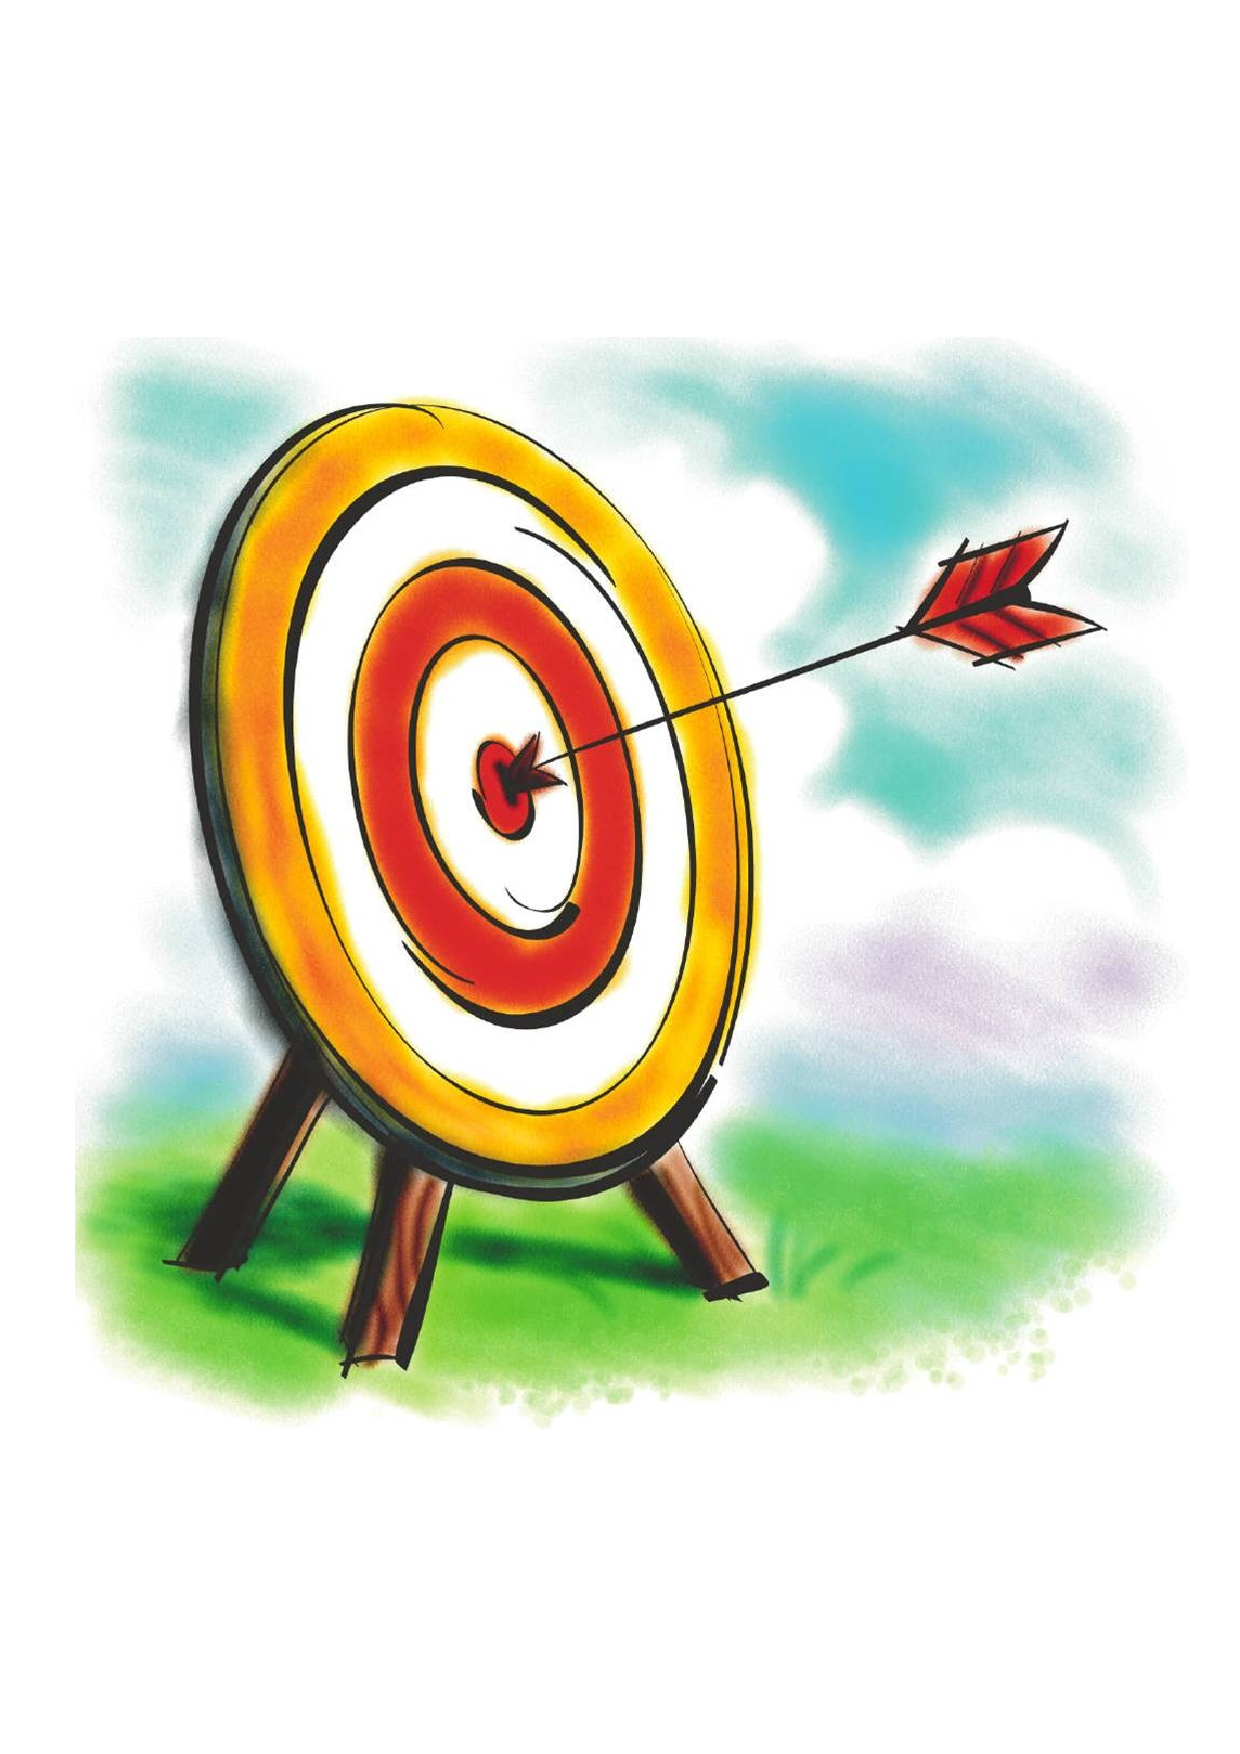
\includegraphics[width=.07\textwidth]{archeryf}}; }
				{\node[fancytitle2,  rounded corners] at (box.west) {\treeBS};}
			}%%
		\end{tikzpicture}
	\end{center}
}%

%%% ============================================================================================

\newcommand{\arcBS}{\noindent\textcolor{red}{\Huge\ding{247}}}
\NewDocumentEnvironment{warning}{g g}{
	\tikzstyle{mybox1} = [draw=red, fill=red!15,very thick, rectangle, rounded corners, inner sep=10pt, inner ysep=20pt]
	\tikzstyle{fancytitle1} =[fill=red!90, text=white]
	\tikzstyle{fancytitle2} =[fill=red!4, text=white]
	\tikzstyle{fancytitle3} =[fill=white, text=white]
	\begin{flushleft}
	\begin{tikzpicture}
	\node [mybox1] (box)\bgroup
	\IfValueTF{#2}{
		\IfFileExists{#2}{\begin{minipage}{.85\textwidth}}{\begin{minipage}{.93\textwidth}}
	}{%%
		\IfFileExists{warining.png}{\begin{minipage}{.85\textwidth}}{\begin{minipage}{.93\textwidth}}
	}%%
	\baselineskip=.95cm
		\begin{RTL}
}{%
		\end{RTL}
	\end{minipage}
	\egroup;
	\IfValueTF{#1}{\node[fancytitle1, left=10pt] at (box.north east) {\hboxR{#1}};}{\node[fancytitle1, left=10pt] at (box.north east) {\hboxR{توجه}};}%
	\IfValueTF{#2}{
		\IfFileExists{#2}
		{\node[fancytitle3, left=3pt,   rounded corners] at (box.west) {\includegraphics[width=.07\textwidth]{#2}}; }
		{\node[fancytitle2,  rounded corners] at (box.west) {\arcBS};}			
	}{%%
		\IfFileExists{warining.png}
		{\node[fancytitle3, left=3pt,   rounded corners] at (box.west) {
\includegraphics[width=.07\textwidth]{warining.png}}; }
		{\node[fancytitle2,  rounded corners] at (box.west) {\arcBS};}
	}%%
	\end{tikzpicture}
	\end{flushleft}
}%

%%% ============================================================================================

\newcommand{\envBS}{\noindent\textcolor{Violet}{\Huge\ding{41}}}
\NewDocumentEnvironment{refer}{g g}{
	\tikzstyle{mybox1} = [draw=Violet, fill=Violet!10,very thick, rectangle, rounded corners, inner sep=10pt, inner ysep=20pt]
	\tikzstyle{fancytitle1} =[fill=Violet!50, text=white]
	\tikzstyle{fancytitle2} =[fill=Violet!20, text=white]
	\tikzstyle{fancytitle3} =[fill=white, text=white]
	\begin{flushleft}
	\begin{tikzpicture}
	\node [mybox1] (box)\bgroup
	\IfValueTF{#2}{
		\IfFileExists{#2}{\begin{minipage}{.85\textwidth}}{\begin{minipage}{.93\textwidth}}
	}{%%
		\IfFileExists{referO.pdf}{\begin{minipage}{.85\textwidth}}{\begin{minipage}{.93\textwidth}}
	}%%
	\baselineskip=.95cm
	\begin{RTL}
}{%
	\end{RTL}
	\end{minipage}
	\egroup;
	\IfValueTF{#1}{\node[fancytitle1, left=10pt] at (box.north east) {\hboxR{#1}};}{\node[fancytitle1, left=10pt] at (box.north east) {\hboxR{مراجع مفید}};}%
	\IfValueTF{#2}{
		\IfFileExists{#2}
		{\node[fancytitle3, left=3pt,   rounded corners] at (box.west) {\includegraphics[width=.07\textwidth]{#2}}; }
		{\node[fancytitle2,  rounded corners] at (box.west) {\envBS};}			
	}{%%
		\IfFileExists{referO.pdf}
		{\node[fancytitle3, left=3pt,   rounded corners] at (box.west) {
\includegraphics[width=.07\textwidth]{referO}}; }
		{\node[fancytitle2,  rounded corners] at (box.west) {\envBS};}
	}%%
	\end{tikzpicture}
	\end{flushleft}
}%

\newcommand{\goodRef}[1]{ \begin{refer} #1 \end{refer} }

%%% ============================================================================================

\newcommand{\twoBS}{\noindent\textcolor{YellowOrange}{\Huge\ding{44}}}
\NewDocumentEnvironment{info}{g g}{
	\tikzstyle{mybox1} = [draw=YellowOrange, fill=YellowOrange!10,very thick, rectangle, rounded corners, inner sep=10pt, inner ysep=20pt]
	\tikzstyle{fancytitle1} =[fill=YellowOrange!50, text=white]
	\tikzstyle{fancytitle2} =[fill=YellowOrange!15, text=white]
	\tikzstyle{fancytitle3} =[fill=white, text=white]
	\begin{flushleft}
	\begin{tikzpicture}
	\node [mybox1] (box)\bgroup
	\IfValueTF{#2}{
		\IfFileExists{#2}{\begin{minipage}{.85\textwidth}}{\begin{minipage}{.93\textwidth}}
	}{
		\IfFileExists{infoRR.png}{\begin{minipage}{.85\textwidth}}{\begin{minipage}{.93\textwidth}}
	}%%
	\baselineskip=.95cm
	\begin{RTL}
}{%
	\end{RTL}
	\end{minipage}
	\egroup;
	\IfValueTF{#1}{\node[fancytitle1, left=10pt] at (box.north east) {\hboxR{#1}};}{\node[fancytitle1, left=10pt] at (box.north east) {\hboxR{مطالب بیشتر}};}%%
	\IfValueTF{#2}{
		\IfFileExists{#2}
		{\node[fancytitle3, left=3pt,   rounded corners] at (box.west) {\includegraphics[width=.07\textwidth]{#2}}; }
		{\node[fancytitle2,  rounded corners] at (box.west) {\twoBS};}			
	}{
		\IfFileExists{infoRR.png}
		{\node[fancytitle3, left=3pt,   rounded corners] at (box.west) {
\includegraphics[width=.07\textwidth]{infoRR}}; }
		{\node[fancytitle2,  rounded corners] at (box.west) {\twoBS};}
	}%%
	\end{tikzpicture}
	\end{flushleft}
}%

%%% ============================================================================================


\newcommand{\teleBS}{\noindent\textcolor{Mulberry}{\Huge\ding{37}}}
\NewDocumentEnvironment{problem}{g g}{
	\tikzstyle{mybox1} = [draw=Mulberry, fill=Mulberry!10,very thick, rectangle, rounded corners, inner sep=10pt, inner ysep=20pt]
	\tikzstyle{fancytitle1} =[fill=Mulberry!50, text=white]
	\tikzstyle{fancytitle2} =[fill=Mulberry!15, text=white]
	\tikzstyle{fancytitle3} =[fill=white, text=white]
	\begin{flushleft}
	\begin{tikzpicture}
	\node [mybox1] (box)\bgroup
	\IfValueTF{#2}{
		\IfFileExists{#2}{\begin{minipage}{.85\textwidth}}{\begin{minipage}{.93\textwidth}}
	}{
		\IfFileExists{home.png}{\begin{minipage}{.85\textwidth}}{\begin{minipage}{.93\textwidth}}
	}%%
	\baselineskip=\baselineskipVar
	\begin{RTL}
}{%
	\end{RTL}
	\end{minipage}
	\egroup;
	\IfValueTF{#1}{\node[fancytitle1, left=10pt] at (box.north east) {\hboxR{#1}};}{\node[fancytitle1, left=10pt] at (box.north east) {\hboxR{سوال}};}%%
	\IfValueTF{#2}{
		\IfFileExists{#2}
		{\node[fancytitle3, left=3pt,   rounded corners] at (box.west) {\includegraphics[width=.07\textwidth]{#2}}; }
		{\node[fancytitle2,  rounded corners] at (box.west) {\twoBS};}			
	}{
		\IfFileExists{home.png}
		{\node[fancytitle3, left=3pt,   rounded corners] at (box.west) {
\includegraphics[width=.07\textwidth]{home}}; }
		{\node[fancytitle2,  rounded corners] at (box.west) {\teleBS};}
	}%%
	\end{tikzpicture}
	\end{flushleft}
}%


%%% =========================================================================================================

\newcommand{\defBS}{\noindent\textcolor{ForestGreen}{\Huge\ding{45}}}
\NewDocumentEnvironment{mydef}{g g}{
	\tikzstyle{mybox1} = [draw=Plum, fill=Plum!15,very thick, rectangle, rounded corners, inner sep=10pt, inner ysep=20pt]
	\tikzstyle{fancytitle1} =[fill=Plum, text=white]
	\tikzstyle{fancytitle2} =[fill=Plum!5, text=white]
	\tikzstyle{fancytitle3} =[fill=white, text=white]
	\begin{center}
		\begin{tikzpicture}
			\node [mybox1] (box)\bgroup
			\IfValueTF{#2}{
				\IfFileExists{#2}{\begin{minipage}{.85\textwidth}}{\begin{minipage}{.93\textwidth}}
			}{%%
				\IfFileExists{defi.png}{\begin{minipage}{.85\textwidth}}{\begin{minipage}{.93\textwidth}}
			}%%
			\baselineskip=.95cm
				\begin{RTL}
}{%
				\end{RTL}
			\end{minipage}
			\egroup;
			\IfValueTF{#1}{\node[fancytitle1, left=10pt] at (box.north east) {\hboxR{#1}};}{\node[fancytitle1, left=10pt] at (box.north east) {\hboxR{تعریف}};}%
			\IfValueTF{#2}{
				\IfFileExists{#2}
				{\node[fancytitle3, left=3pt,   rounded corners] at (box.west) {\includegraphics[width=.07\textwidth]{#2}}; }
				{\node[fancytitle2,  rounded corners] at (box.west) {\defBS};}			
			}{%%
				\IfFileExists{defi.png}
				{\node[fancytitle3, left=3pt,   rounded corners] at (box.west) {
\includegraphics[width=.07\textwidth]{defi}}; }
				{\node[fancytitle2,  rounded corners] at (box.west) {\defBS};}
			}%%
		\end{tikzpicture}
	\end{center}
}%

%%% =========================================================================================================

\newcommand{\commentBSS}{\noindent\textcolor{ForestGreen}{\Huge\ding{23}}}
\NewDocumentEnvironment{mycomment}{g g}{
	\tikzstyle{mybox1} = [draw=red,fill=none,very thick, rectangle, rounded corners, inner sep=10pt, inner ysep=20pt]
	\tikzstyle{fancytitle1} =[fill=red, text=white]
	\tikzstyle{fancytitle2} =[fill=red!5, text=white]
	\tikzstyle{fancytitle3} =[fill=white, text=white]
	\begin{center}
		\begin{tikzpicture}
			\node [mybox1] (box)\bgroup
			\IfValueTF{#2}{
				\IfFileExists{#2}{\begin{minipage}{.85\textwidth}}{\begin{minipage}{.93\textwidth}}
			}{%%
				\IfFileExists{robah.png}{\begin{minipage}{.85\textwidth}}{\begin{minipage}{.93\textwidth}}
			}%%
			\baselineskip=.95cm
				\begin{RTL}
}{%
				\end{RTL}
			\end{minipage}
			\egroup;
			\IfValueTF{#1}{\node[fancytitle1, left=10pt] at (box.north east) {\hboxR{#1}};}{\node[fancytitle1, left=10pt] at (box.north east) {\hboxR{توضیح}};}%
			\IfValueTF{#2}{
				\IfFileExists{#2}
				{\node[fancytitle3, left=3pt,   rounded corners] at (box.west) {\includegraphics[width=.07\textwidth]{#2}}; }
				{\node[fancytitle2,  rounded corners] at (box.west) {\commentBSS};}			
			}{%%
				\IfFileExists{robah.png}
				{\node[fancytitle3, left=3pt,   rounded corners] at (box.west) {
\includegraphics[width=.07\textwidth]{robah}}; }
				{\node[fancytitle2,  rounded corners] at (box.west) {\commentBSS};}
			}%%
		\end{tikzpicture}
	\end{center}
}%

%%% =========================================================================================================



\newtheoremstyle{ntdefinitionstyle}% name of the style to be used
  {\topsep}% measure of space to leave above the theorem. E.g.: 3pt
  {\topsep}% measure of space to leave below the theorem. E.g.: 3pt
  {}% name of font to use in the body of the theorem
  {0pt}% measure of space to indent
  {\bfseries\color{nttitle}}% name of head font
  {}% punctuation between head and body
  {.5em}% space after theorem head; " " = normal interword space
  {}% Manually specify head  

\newtheoremstyle{nttheoremstyle}% name of the style to be used
  {\topsep}% measure of space to leave above the theorem. E.g.: 3pt
  {\topsep}% measure of space to leave below the theorem. E.g.: 3pt
  {}% name of font to use in the body of the theorem
  {0pt}% measure of space to indent
  {\bfseries\color{nttitle}}% name of head font
  {}% punctuation between head and body
  {.2em}% space after theorem head; " " = normal interword space
  {}% Manually specify head
  
\newtheoremstyle{ntplainstyle}% name of the style to be used
  {\topsep}% measure of space to leave above the theorem. E.g.: 3pt
  {\topsep}% measure of space to leave below the theorem. E.g.: 3pt
  {\itshape}% name of font to use in the body of the theorem
  {0pt}% measure of space to indent
  {\bfseries\color{nttitle}}% name of head font
  {}% punctuation between head and body
  {.5em}% space after theorem head; " " = normal interword space
  {}% Manually specify head  



\definecolor{nttitle}{RGB}{0,177,235}
% رنگ آبی کم‌رنگ پس‌زمینه محیط قضیه و محیط lstlisting
\definecolor{ntback}{RGB}{212,237,255}
% رنگ سبز صفحه عنوان فارسی و انگلیسی کتاب، قسمت‌ها و محیط ntpoint
\definecolor{ntsec}{RGB}{204,233,157}
% رنگ قهوه‌ای محیط تعریف
\definecolor{ntdef}{RGB}{205,0,205}

\definecolor{ntexp}{RGB}{224,110,12}


\mdfdefinestyle{theoremstyle}{%
hidealllines=true,
frametitlerule=false,
innerrightmargin=5pt,
innerleftmargin=5pt,
frametitlerulewidth=0pt,
frametitlefont=\color{white}\large\bfseries,
linewidth=2pt,%
frametitlerule=true,%
frametitlebackgroundcolor=nttitle,
innertopmargin=\topskip,
skipabove=.7\baselineskip,
skipbelow=1.8\baselineskip,
backgroundcolor=nttitle!15,
startinnercode={\baselineskip=.9cm},
startcode={\vspace{.8\topsep}},
splitbottomskip=10pt,
theoremseparator={},
needspace=4\baselineskip
align=center,
}
\mdtheorem[style=theoremstyle]{nttheorem}[theorem]{\hspace*{1pt}قضیه}


\newcounter{ntcounter}
\makeatletter
\renewcommand\thentcounter{\thechapter\@SepMark\arabic{ntcounter}} 
\newenvironment{ntpoint}[1][\empty]{\par\begin{mdframed}[
hidealllines=true,
innertopmargin=9pt,
skipabove=.9\baselineskip,
innermargin=\dimexpr-\marginparwidth-\marginparsep\relax,
innerbottommargin=9pt,
innerrightmargin=5pt,innerleftmargin=5pt,
backgroundcolor=ntsec,
  singleextra={
      \node[
        overlay,
        inner ysep=7pt,
       inner xsep=9pt,
        anchor=east,
       % text width=1.2cm,
       % align=left,
        minimum height=4ex,
        fill=nttitle,
        yshift=-5.2mm,
        xshift=0mm,
        %rounded corners=3pt,
        font=\color{white}\bfseries
      ] at (P) {\rl{نکته~\thentcounter}};
        \draw[white,fill=white] ($(P)-(0pt,1.65mm)$) -- ($(P)-(0pt,8.8mm)$) -- ($(P)-(7pt,5.225mm)$) -- cycle;
      },
   firstextra={
      \node[
       overlay,
        inner ysep=7pt,
       inner xsep=9pt,
        anchor=east,
       % text width=1.2cm,
       % align=left,
        minimum height=4ex,
        fill=nttitle,
        yshift=-5.2mm,
        xshift=0mm,
        %rounded corners=3pt,
        font=\color{white}\bfseries
      ] at (P) {\rl{نکته~\thentcounter}};
        \draw[white,fill=white] ($(P)-(0pt,1.65mm)$) -- ($(P)-(0pt,8.8mm)$) -- ($(P)-(7pt,5.225mm)$) -- cycle;
      },
]\baselineskip=\baselineskipVar\refstepcounter{ntcounter}
\textbf{\ifx\empty#1\hspace*{1.9cm}\relax\else\hspace*{1.65cm}(#1)\fi}%\\[.2cm]%
\noindent\ignorespaces%
\noindent}{\end{mdframed}\par\vspace*{.4ex}}
\@addtoreset{ntcounter}{chapter}
\makeatother


%%%%%%%%%%%%%%%%%%%%%%%%%%%%%%%%%%%%%%%%%%%%%%%%%
% تعریف محیط ntexample


\newcounter{ntexample}
\makeatletter
\renewcommand\thentexample{\thechapter\@SepMark\arabic{ntexample}} 

\newenvironment{ntexample}[1][\empty]{\par\begin{mdframed}[roundcorner=10pt,,align=right,skipabove=.5\baselineskip,
skipbelow=.3\baselineskip,
innertopmargin=10pt,
innerbottommargin=12pt,
usetwoside=false,
innerrightmargin=10pt,
rightmargin=3pt,
innerleftmargin=0pt,
%outermargin=1pt,
%backgroundcolor=brown!25,
 topline=false,bottomline=false,leftline=false,
middlelinewidth=8pt,
%splittopskip=-15pt,
splitbottomskip=5pt,
middlelinecolor=ntexp,
  singleextra={
      \node[
        overlay,
        outer sep=0pt,
        anchor=north west,
        text width=2.1cm,
        minimum height=4ex,
        fill=ntexp,
        yshift=-2mm,
        xshift=-21mm,
        %rounded corners=3pt,
        font=\color{white}\bfseries
      ] at (P) {\rl{مثال~\thentexample}};
      },
   firstextra={
      \node[
        overlay,
        outer sep=0pt,
        anchor=north west,
        text width=2.1cm,
        minimum height=4ex, 
        fill=ntexp,
        yshift=-2mm,
        xshift=-21mm,
        %rounded corners=3pt,
        font=\color{white}\bfseries
      ] at (P) {\rl{مثال~\thentexample}};
      },
]
\baselineskip=\baselineskipVar
\refstepcounter{ntexample}
\hspace*{1.8cm}\textbf{\ifx\empty#1\space\relax\else\space\textcolor{nttitle}{#1}\space \ \fi}%\\[.2cm]%
%\noindent\ignorespaces%
}{\end{mdframed}\par}
\@addtoreset{ntexample}{chapter}
\makeatother


\newenvironment{ntexample2}[1][\empty]{\par\begin{mdframed}[roundcorner=10pt,,align=right,skipabove=.5\baselineskip,
skipbelow=.3\baselineskip,
innertopmargin=10pt,
innerbottommargin=12pt,
usetwoside=false,
innerrightmargin=10pt,
rightmargin=3pt,
innerleftmargin=0pt,
%outermargin=1pt,
%backgroundcolor=brown!25,
 topline=false,bottomline=false,leftline=false,
middlelinewidth=8pt,
%splittopskip=-15pt,
splitbottomskip=5pt,
middlelinecolor=ntexp,
  singleextra={
      \node[
        overlay,
        outer sep=0pt,
        anchor=north west,
        text width=2.1cm,
        minimum height=4ex,
        fill=ntexp,
        yshift=-2mm,
        xshift=-21mm,
        %rounded corners=3pt,
        font=\color{white}\bfseries
      ] at (P) {\rl{مثال}};
      },
   firstextra={
      \node[
        overlay,
        outer sep=0pt,
        anchor=north west,
        text width=2.1cm,
        minimum height=4ex, 
        fill=ntexp,
        yshift=-2mm,
        xshift=-21mm,
        %rounded corners=3pt,
        font=\color{white}\bfseries
      ] at (P) {\rl{مثال}};
      },
]
\baselineskip=\baselineskipVar
\hspace*{1.8cm}\textbf{\ifx\empty#1\space\relax\else\space\textcolor{nttitle}{#1}\space \ \fi}%\\[.2cm]%
%\noindent\ignorespaces%
}{\end{mdframed}\par}
\makeatother

\makeatletter
\newenvironment{ntremember}[1][\empty]{\par\begin{mdframed}[roundcorner=10pt,,align=right,skipabove=.5\baselineskip,
skipbelow=.3\baselineskip,
innertopmargin=10pt,
innerbottommargin=12pt,
usetwoside=false,
innerrightmargin=10pt,
rightmargin=3pt,
innerleftmargin=0pt,
%outermargin=1pt,
%backgroundcolor=brown!25,
 topline=false,bottomline=false,leftline=false,
middlelinewidth=8pt,
%splittopskip=-15pt,
splitbottomskip=5pt,
middlelinecolor=ForestGreen,
  singleextra={
      \node[
        overlay,
        outer sep=0pt,
        anchor=north west,
        text width=2.1cm,
        minimum height=4ex,
        fill=ForestGreen,
        yshift=-2mm,
        xshift=-21mm,
        %rounded corners=3pt,
        font=\color{white}\bfseries
      ] at (P) {\rl{یادآوری}};
      },
   firstextra={
      \node[
        overlay,
        outer sep=0pt,
        anchor=north west,
        text width=2.1cm,
        minimum height=4ex, 
        fill=ForestGreen,
        yshift=-2mm,
        xshift=-21mm,
        %rounded corners=3pt,
        font=\color{white}\bfseries
      ] at (P) {\rl{یادآوری}};
      },
]
\baselineskip=\baselineskipVar
\hspace*{1.8cm}\textbf{\ifx\empty#1\space\relax\else\space\textcolor{nttitle}{#1}\space \ \fi}%\\[.2cm]%
%\noindent\ignorespaces%
}{\end{mdframed}\par}
\makeatother


\newenvironment{ntdefinition}[1][\empty]{\par\begin{mdframed}[roundcorner=10pt,,align=right,skipabove=.5\baselineskip,
skipbelow=.5\baselineskip,
innertopmargin=10pt,
innerbottommargin=0pt,
usetwoside=false,
innerrightmargin=10pt,
rightmargin=3pt,
innerleftmargin=0pt,
%outermargin=1pt,
%backgroundcolor=brown!25,
 topline=false,bottomline=false,leftline=false,
middlelinewidth=8pt,
%splittopskip=-15pt,
splitbottomskip=5pt,
middlelinecolor=ntdef,
  singleextra={
      \node[
        overlay,
        outer sep=0pt,
        anchor=north west,
        text width=2.1cm,
        minimum height=4ex,
        fill=ntdef,
        yshift=-2mm,
        xshift=-21mm,
        %rounded corners=3pt,
        font=\color{white}\bfseries
      ]     at (P) {\rl{تعریف~\thedefinition}};
      },
   firstextra={
      \node[
        overlay,
        outer sep=0pt,
        anchor=north west,
        text width=2.1cm,
        minimum height=4ex, 
        fill=ntdef,
        yshift=-2mm,
        xshift=-21mm,
        %rounded corners=3pt,
        font=\color{white}\bfseries
      ] at (P) {\rl{تعریف~\thedefinition}};
      },
]
\baselineskip=\baselineskipVar
\refstepcounter{definition}
\hspace*{1.8cm}\textbf{\ifx\empty#1\space\relax\else\space\textcolor{nttitle}{#1}\space \ \fi}%
%\noindent\ignorespaces%
}{\end{mdframed}\hspace*{1.5cm} \par}

%%%%%%%%%%%%%%%%%%%%%%%%%%%%%%%%%%%%%%%%%%%%%%%%%
% تعریف محیط ntsolution
\newenvironment{ntsolution}{\par\begin{mdframed}[skipabove=.7\baselineskip,
innertopmargin=0pt,
innerbottommargin=0pt,
innerrightmargin=8pt,innerleftmargin=0pt,
outermargin=-1pt,
%backgroundcolor=green,
 topline=false,bottomline=false,leftline=false,
middlelinewidth=8pt,
middlelinecolor=nttitle,
]
\baselineskip=\baselineskipVar
\textbf{\textcolor{nttitle}{حل}}\ \
\noindent}{\end{mdframed}\par}

%%%%%%%%%%%%%%%%%%%%%%%%%%%%%%%%%%%%%%%%%%%%%%%%%
% تعریف محیط ntproblems برای حروف‌چینی تمرین‌های پایان فصل‌ها
\makeatletter
\newenvironment{ntproblems}[1][تمرین‌ها]{%
\renewcommand{\thesection}{}
\phantomsection\addcontentsline{toc}{section}{\hspace*{2pt}#1}
\vspace*{.7\baselineskip}
\needspace{5\baselineskip}
\begin{fullwidth}
\par
\begin{mdframed}[%outermargin=\dimexpr-\marginparwidth-\marginparsep\relax,align=center,%skipabove=.7\baselineskip,
%skipbelow=.1\baselineskip,
innertopmargin=9pt,
innerbottommargin=9pt,
%outermargin=-5pt,
usetwoside=false,
rightmargin=0pt,
innerrightmargin=5pt,innerleftmargin=0pt,
backgroundcolor=nttitle!15,
topline=false,
bottomline=false,leftline=false,
middlelinewidth=20pt,
middlelinecolor=nttitle,
]
\normalfont\Large\bfseries #1
\end{mdframed}%
\end{fullwidth}
\vspace*{-.5\baselineskip}
\sectionmark{#1}
\renewcommand\theenumi{\color{nttitle}\bfseries\thechapter\@SepMark\arabic{enumi}}
\renewcommand\labelenumi{\theenumi}
\let\p@enumii\@empty
\setlength{\columnsep}{5ex}
\begin{adjmulticols*}{2}{-\dimexpr+\marginparwidth+\marginparsep\relax}{}
\begin{enumerate}[align=left,itemindent=0pt,labelwidth=5ex,leftmargin=6ex
]}
{\end{enumerate}
\raggedcolumns
\end{adjmulticols*}
}  
\makeatother

%%%%%%%%%%%%%%%%%%%%%%%%%%%%%%%%%%%%%%%%%%%%%%%%%
% تعریف محیط ntsolutions برای حروف‌چینی پاسخ تمرین‌ها
\newenvironment{ntsolutions}{%
\setlength{\columnsep}{5ex}
\begin{adjmulticols*}{2}{-\dimexpr+\marginparwidth+\marginparsep\relax}{}
}
{
\raggedcolumns
\end{adjmulticols*}
}  

%%%%%%%%%%%%%%%%%%%%%%%%%%%%%%%%%%%%%%%%%%%%%%%%%
% تعریف دستور ntchsol برای مشخص کردن پاسخ‌های مربوط به هر فصل در محیط ntsolutions
\newcommand{\ntchsol}[1]{
%\vspace*{.7\baselineskip}
%\needspace{4\baselineskip}
\par
\begin{mdframed}[%outermargin=\dimexpr-\marginparwidth-\marginparsep\relax,align=center,
skipabove=.7\baselineskip,
%skipbelow=.1\baselineskip,
innertopmargin=9pt,
innerbottommargin=9pt,
%outermargin=-5pt,
usetwoside=false,
rightmargin=0pt,
innerrightmargin=5pt,innerleftmargin=0pt,
backgroundcolor=nttitle!15,
topline=false,
bottomline=false,leftline=false,
middlelinewidth=20pt,
middlelinecolor=nttitle,
]
\normalfont\Large\bfseries #1
\end{mdframed}%
%\end{fullwidth}
\vspace*{-.5\baselineskip}
}

%%%%%%%%%%%%%%%%%%%%%%%%%%%%%%%%%%%%%%%%%%%%%%%%%

\def\lemmaautorefname{لم}












% فایل  ChapterStyle  در برگیرنده تعریف یکسری استایل برای فصل‌ها است. 
%% Last Update: 24 Jul 2019
%

%% =========================================================================================================================
% انواع مختلف استایل‌های برای عنوان فصل‌ها 

\newcommand*\chapterlabel{}
\titleformat{\chapter}
  {\gdef\chapterlabel{}
   \normalfont\Huge\bfseries}
  {\gdef\chapterlabel{\thechapter\ }}{0pt}
  {\begin{tikzpicture}[remember picture,overlay]
    \node[yshift=-3cm] at (current page.north west)
      {\begin{tikzpicture}[remember picture, overlay]
        \draw[fill=BlueGreen] (0,0) rectangle
          (\paperwidth,3cm);
        \setRTL
        \node[anchor=east,xshift=0.95\paperwidth,rectangle,
              rounded corners=20pt,inner sep=11pt,
              fill=MidnightBlue,text width=\dimexpr0.9\paperwidth-22pt\relax,align=justify]
             {\addfontfeature{Color=F5F5F5}\chapterlabel#1};
       \end{tikzpicture}
      };
   \end{tikzpicture}
  }
%\titlespacing*{\chapter}{0pt}{50pt}{-60pt}
\makeatletter
\bidi@patchcmd{\@makechapterhead}%
{\huge\bfseries\@chapapp\space\thechapter}%
{}%
{}
{}

\bidi@patchcmd{\@chapter}%
{\addcontentsline{toc}{chapter}{\protect\numberline{\thechapter}#1}}%
{\addcontentsline{toc}{chapter}{#1}}%
{}
{}

\bidi@patchcmd{\@part}{%
  \addcontentsline{toc}{part}{\thepart\hspace{1em}#1}%%
}{%
  \addtocontents{toc}{\bfseries\protect\centering\thepart\hspace{1em}#1\par}%
}{}{}
\makeatother


% تعریف یکسری استایل برای صفحه شروع 
%% Last Update: 20 Sep 2019
%

%% =================================================================================
\makeatletter
% تعریف یکسری متغیرها که کاربر می‌تواند بعدا آن ها را مقداردهی کند. 

\gdef\@type{نوع پروژه}
\def\type#1{\gdef\@type{#1}}

% عنوان محصول را تعیین می‌کند. این عنواند در ایجاد عنوان در مستند استفاده می‌شود این عنوان در هر مستند باید ایجاد شود در غیر این صورت از عنوان پیشفرض استفاده خواهد شد.
\gdef\@title{عنوان پروژه}
\def\title#1{\gdef\@title{#1}}

% زیر عنوان یک متن ساده را تعیین می‌کند که یک هدف مهم محصول را تعیین می‌کند این عنوان می تواند برای یک محصول در نظر گرفته نشود. از این داده برای  ایجاد عنوان و سایر مکان های محصول استفاده می‌شود.
\gdef\@subtitle{کاربرد محصول برای استفاده در زیر عنوان}
\def\subtitle#1{\gdef\@subtitle{#1}}
% افراد و گروه های که در تهیه این مستند و محصول همکاری داشته اند را تعیین می کند این داده همواره باید بیان شود. این داده در نوشتن عنوان و دیگر قسمت های مستند مورد استفاده قرار می‌گیرد.
\gdef\@author{}
\def\author#1{\gdef\@author{#1}}
\newcommand{\authorText}{\@author\,}
% تاریخ نهایی نوشتن مستند را تعیین می‌کند این تاریخ در نوشتن عنوان استفاده می‌شود این تارخ باید تعیین شود در غیر این صورت به صورت پیش فرض یک تاریخ برای آن استفاده می شود.
\gdef\@date{ آخرین ویرایش: \myData}
\def\date#1{\gdef\@date{#1}}

\gdef\@supervisor{} 
\def\supervisor#1{\gdef\@supervisor{#1}}
\newcommand{\supervisorText}{\@supervisor\,}

\gdef\@adviser{نام استاد مشاور}
\def\adviser#1{\gdef\@adviser{#1}}

\gdef\@session{جلسه ارایه}
\def\session#1{\gdef\@session{#1}}

\gdef\@institute{پژوهشکده}
\def\institute#1{\gdef\@institute{#1}}

\gdef\@faculity{ نام دانشکده}
\def\faculity#1{\gdef\@faculity{#1}}

\gdef\@group{ نام گروه}
\def\group#1{\gdef\@group{#1}}

\gdef\@community{نام زیرگروه}
\def\community#1{\gdef\@community{#1}}

\gdef\@forwhat{پایان‌نامه یا رساله برای دریافت درجه}
\def\forwhat#1{\gdef\@forwhat{#1}}

\gdef\@field{در رشته مهندسی کامپیوتر گرایش}
\def\field#1{\gdef\@field{#1}}

\gdef\@version{اول}
\def\version#1{\gdef\@version{#1}}

% نام فایلی لوگوی مورد استفاده در نوشتار توسط این پارامتر مشخص می‌شود. 
\gdef\@logofile{logonotfound}
\def\logofile#1{\gdef\@logofile{#1}}
% اندازه فایل لوگوی موجود در متن توسط این پارامتر مشخص می‌شود.
\gdef\@logoScale{.3\textwidth}
\def\logoScale#1{\gdef\@logoScale{#1}}


%% ============================================================================================================================
%  برگه نخست در مستند را ایجاد می‌کند. در این برگه تنها نام پروردگار  ذکر می‌شود. برای ایجاد نام پرودگار یک تصویر استفاده می‌شود به نام god.ps  که باید در پوشه image کنار پرونده اصلی مستند قرار گرفته شده باشد.
\deflatinfont\besm[Scale=50]{Besmellah 2}
\DeclareDocumentCommand{\Godpage}{g g}{	
	\thispagestyle{empty}
	\begin{center}
	\IfValueTF{#1}{
		\IfValueTF{#2}{
			\includegraphics[width=#2\textwidth]{#1}
		}{%
			\includegraphics[width=.7\textwidth]{#1}
		}%
	}{%%
		\IfValueTF{#2}{
			{\besm #2}
		}{%
			{\besm b}

		}%
	}%%
	\end{center}
	\newpage
}%

\DeclareDocumentCommand{\Godpage}{g}{	
	\thispagestyle{empty}
	\begin{center}
		\IfValueTF{#1}{
			{\besm #1}
		}{%
			{\besm f}

		}%
	\end{center}
	\newpage
}%

\DeclareDocumentCommand{\GodpageFont}{gg}{	
	\thispagestyle{empty}
	\begin{center}
		\IfValueTF{#1}{
			\IfValueTF{#2}{
			}{%
			}%
			{\besm بسم‌الله الرحمن الرحیم}
		}{%
			{\besm بسم‌الله الرحمن الرحیم}

		}%
	\end{center}
	\newpage
}%


%% ============================================================================================================================

\newcommand{\pejoheshStyle}{
% این یک استایل ساده و رسمی.
% توسط این دستور تمامی footer و header های صفحه را حذف می‌کنیم. 
	\thispagestyle{empty}
	\begin{center}
		\includegraphics[width=\@logoScale]{\@logofile}\\*[10pt]
		\logofontR{\@institute}\medskip
		\vspace*{\stretch{2}}
		\typefontR\textbf{\@type}\\*[35pt]
		\titlefontR\textbf{\@title}\medskip
		\vspace*{\stretch{2}}
		\datafontR{\@author}\medskip
		\vspace*{\stretch{2}}
		\datafontR{\@date}
		\vspace*{\stretch{1}}
	\end{center}
	\clearpage
} %


%% ============================================================================================================================
% توسط دستورات defpersianfont و deflatinfont به ترتیب می توان یکسری فونت فارسی و انگلیسی دیگر تعریف کرد که در جاهای دیگر متن بتوان از آن استفاده کرد. برای استفاده کافی است که عبارتی که می خواهیم فونت آن عوض شود را به صورت زیر به عنوان نمونه بنویسیم.
\defpersianfont\titlefont[Scale=2.4]{IRTitr}
\newcommand{\lshortStyle}{
% استایلی شبیه به استایل شروع کتاب "مقدمه‌ای نه چندان کوتاه بر Latex"
	\definecolor{authorcol}{rgb}{.51,0,.51}
	\begin{flushleft}
	\vspace*{\stretch{.1}}
	\begin{flushright}\includegraphics[width=\@logoScale]{\@logofile}\end{flushright}
	\newlength{\centeroffset}
	\setlength{\centeroffset}{-0.5\oddsidemargin}
	\addtolength{\centeroffset}{0.5\evensidemargin}
	\addtolength{\textwidth}{-\centeroffset}
% توسط این دستور تمامی footer و header های صفحه را حذف می‌کنیم. 
	\thispagestyle{empty}
	
	\vspace*{\stretch{2}}
	
	\noindent\hspace*{\centeroffset}\makebox[0pt][l]{
		\begin{minipage}{\textwidth}
			\flushleft
			{ \titlefont\textcolor{magenta}\@title \\*[10pt]}
			\noindent\color{gray}{\rule[-1ex]{\textwidth}{5pt}\\*[4mm]
			\hfill{\large \bfseries\@type }}
		\end{minipage}
	}%
	
	\vspace{\stretch{2}}
	
	\noindent\hspace*{\centeroffset}\makebox[0pt][l]{
		\begin{minipage}{\textwidth}
			{\flushleft\textcolor{authorcol}{\bfseries\@author\\*[5pt]}}
			{\flushleft\textcolor{authorcol}{\bfseries\@supervisor\\*[5pt]}}
			{\flushleft\textcolor{authorcol}{\bfseries\small\@date}\\}
		\end{minipage}
	}%
		
	\vspace{\stretch{1.5}}

	\end{flushleft}
	\clearpage
}%

%% ===============================================================================

%\newfontfamily\sols[Scale=2.5,Script=Parsi,Language=Parsi,Mapping=farsidigits]{IranNastaliq}
\newcommand{\presStyle}[1]{
	\defpersianfont\titr[Scale=2]{B Nazanin Outline}

% ایجاد عنوان برای فایل ارایه (Presentation) 
% توسط این دستور تمامی footer و header های صفحه را حذف می‌کنیم. 
	\thispagestyle{empty}
	\deflatinfont\salam[Scale=30]{XB Kayhan}
	\begin{titlepage}
		\centering
		{\salam \textcolor{Blue}{#1}}\\
	   \begin{center}\includegraphics[width=\@logoScale\linewidth]{\@logofile}\end{center}
		\vspace{\stretch{2}}
		\textcolor{Green}{\huge\titr{\@title}}\\
		\vspace{\stretch{2}}
		\textcolor{cyan}{\@session}\\*[14pt]
		\textcolor{cyan}{\@author}\\*[14pt]
		\textcolor{Orange}{\@date}
		\vspace{\stretch{1}}
	\end{titlepage}
	\clearpage\newpage
	\pagestyle{empty}
	\pagenumbering{arabic}
}%	
	

%% ==========================================================================
%استایل مربوط به پایان‌نامه با دو لوگو
\newcommand{\thesisStyleOO}[2]{
	\ignorespaces
	\begin{center}
	\thispagestyle{empty}
	\begin{table}
		\begin{tabular}{ccc}
			\includegraphics[width=.18\textwidth]{#1}
			&
			\begin{minipage}{0.55\linewidth}
				\vskip 0.6cm
				\begin{center}
					\@institute\\* [0.4cm]
					\@faculity\\ [0.4cm]
					\@group \\*[1cm]
				\end{center}
			\end{minipage}
			&
			\includegraphics[width=.2\textwidth]{#2}
		\end{tabular}
	\end{table}
	\vspace*{\stretch{1}}
	\textbf{\LARGE{\@title}}
	\vspace*{\stretch{1}}
	\vskip 1cm
	\large{\@forwhat}\\[.4cm]
	\large{\@field}
	\vspace*{\stretch{1}}
	\vskip 1cm
	\Large{\textbf{\@author}}
	\vskip 1.5cm
	\Large{
	استاد راهنما:}
	 \\ [0.4cm] \Large{\@supervisor}
	\vskip 2cm
	\large{\@date}
	\end{center}
	\clearpage
}%

%% ==============================================================================
%استایل مربوط به پایان‌نامه با یک لوگو
\newcommand{\thesisStyleO}[1]{
\ignorespaces
\begin{center}
\thispagestyle{empty}
\begin{table}
\begin{tabular}{ccc}
& \includegraphics[width=\@logoScale]{\@logofile} & \\
&
\begin{minipage}{0.55\linewidth}
\vskip 0.6cm
\begin{center}
%\@institute\\* [0.4cm]
\@faculity\\ [0.4cm]
\@group \\*[1cm]
\end{center}
\end{minipage}
&
\end{tabular}
\end{table}
\vspace*{\stretch{1}}
\textbf{{\fontsize{15pt}{50pt}\selectfont\@title}}
\vspace*{\stretch{1}}
\vskip 1cm
\large{\@forwhat}\\[.4cm]
	\large{\@field}
	\vspace*{\stretch{1}}
	\vskip 1cm
	\Large{\textbf{\@author}}
	\vskip 1.5cm
	\Large{
	استاد راهنما:}
	 \\ [0.1cm] \Large{\@supervisor}
	\vskip 2cm
	\large{\@date}
	\end{center}
	\clearpage
}%

%% ================================================================================
%استایل مربوط به تکالیف
\newcommand{\homeworkS}{
\thispagestyle{empty}
\begin{center}
\begin{flushright}
\includegraphics[width=\@logoScale]{\@logofile}
\end{flushright}
\vspace{3cm}
{\farsifontshafighT \bfseries {\@title} }
\begin{tikzpicture}
\draw[red,line width=0.15cm](0,0)--(12,0);
\end{tikzpicture} 
\vspace{2cm}
\begin{minipage}{0.8\textwidth}
\begin{flushright} \large
\emph{\textcolor{Plum}{\@author}} \\[0.6cm]
\end{flushright}
\end{minipage}\\[1.5cm]
\begin{minipage}{0.8\textwidth}
\begin{flushright} \large
\emph{\@supervisor}\\[0.6cm]
\end{flushright}
\end{minipage}
\vfill\large \today
\end{center}
\clearpage
}

%% ==================================================================================

\let\oldmaketitle\maketitle
\renewcommand{\maketitle}{
\ifthenelse{\equal{\@titleStyle}{pejohesh}}{\pejoheshStyle}{ %1
\ifthenelse{\equal{\@titleStyle}{lshort}}{\lshortStyle}{ %2
\ifthenelse{\equal{\@titleStyle}{proposal}}{\proposalStyle}{ %3
\ifthenelse{\equal{\@titleStyle}{presentation}}{\presStyle}{ %4
\ifthenelse{\equal{\@titleStyle}{thesis}}{\thesisStyleO}{ %5
\ifthenelse{\equal{\@titleStyle}{homework}}{\homeworkS}{ %6
\oldmaketitle
} %6
} %5
} %4
} %3
}%2
}%1
}%maketitle
\makeatother


%% دستورات لازم برای واژه‌نامه‌ها، فهرست اختصارات و فهرست نمادها در  فایل (Gloss) آورده شده است.
%% Data:  2014-07-23
%% xindy -L persian-variant1 -C utf8 -I xindy -M %.xdy -t %.glg -o %.gls %.glo
%% xindy -L persian-variant1 -C utf8 -I xindy -M %.xdy -t %.blg -o %.bls %.blo
%% xindy -L english -C utf8 -I xindy -M %.xdy -t %.alg -o %.acr %.acn
%%% برای اجرا xindy بر روی فایل .tex و تولید واژه‌نامه‌ها و فهرست اختصارات و فهرست نمادها یکسری  فایل تعریف شده است.‌ Latex داده های مربوط به واژه نامه و .. را در این 
%%%  فایل‌ها نگهداری می‌کند. مهم‌ترین option‌ این قسمت این است که 
%%% عنوان واژه‌نامه‌ها و یا فهرست اختصارات و یا فهرست نمادها را می‌توانید در این‌جا مشخص کنید. 
%%% در این جا عباراتی مثل glg، gls، glo و ... پسوند فایل‌هایی است که برای xindy بکار می‌روند. 
 \newglossary[glg]{english}{gls}{glo}{واژه‌نامه انگلیسی به فارسی}
 \newglossary[blg]{persian}{bls}{blo}{واژه‌نامه فارسی به انگلیسی}
 \makeglossaries
 \glsdisablehyper
 
%%% تعریف استایل برای واژه نامه فارسی به انگلیسی، در این استایل واژه‌های فارسی در سمت راست و واژه‌های انگلیسی در سمت چپ خواهند آمد. از حالت گروه ‌بندی استفاده می‌کنیم، 
%%% یعنی واژه‌ها در گروه‌هایی به ترتیب حروف الفبا مرتب می‌شوند، مثلا:
%%% الف
%%% افتصاد ................................... Economy
%%% اشکال ........................................ Failure
%%% ش
%%% شبکه ...................................... Network
\newglossarystyle{myFaToEn}{%
	\renewenvironment{theglossary}{}{}
	\renewcommand*{\glsgroupskip}{\vskip 10mm}
	\renewcommand*{\glsgroupheading}[1]{\subsection*{\glsgetgrouptitle{##1}}}
	\renewcommand*{\glossentry}[2]{\noindent\glsentryname{##1}\dotfill\space \glsentrytext{##1}
		
	}
}

%% % تعریف استایل برای واژه نامه انگلیسی به فارسی، در این استایل واژه‌های فارسی در سمت راست و واژه‌های انگلیسی در سمت چپ خواهند آمد. از حالت گروه ‌بندی استفاده می‌کنیم، 
%% % یعنی واژه‌ها در گروه‌هایی به ترتیب حروف الفبا مرتب می‌شوند، مثلا:
%% % E
%%% Economy ............................... اقتصاد
%% % F
%% % Failure................................... اشکال
%% %N
%% % Network ................................. شبکه

\newglossarystyle{myEntoFa}{%
	%%% این دستور در حقیقت عملیات گروه‌بندی را انجام می‌دهد. بدین صورت که واژه‌ها در بخش‌های جداگانه گروه‌بندی می‌شوند، 
	%%% عنوان بخش همان نام حرفی است که هر واژه در آن گروه با آن شروع شده است. 
	\renewenvironment{theglossary}{}{}
	\renewcommand*{\glsgroupskip}{\vskip 10mm}
	\renewcommand*{\glsgroupheading}[1]{\begin{LTR} \subsection*{\glsgetgrouptitle{##1}} \end{LTR}}
	%%% در این دستور نحوه نمایش واژه‌ها می‌آید. در این جا واژه فارسی در سمت راست و واژه انگلیسی در سمت چپ قرار داده شده است، و بین آن با نقطه پر می‌شود. 
	\renewcommand*{\glossentry}[2]{\noindent\glsentrytext{##1}\dotfill\space \glsentryname{##1}
		
	}
}

%%% تعیین استایل برای فهرست اختصارات
\newglossarystyle{myAbbrlist}{%
	%%% این دستور در حقیقت عملیات گروه‌بندی را انجام می‌دهد. بدین صورت که اختصارات‌ در بخش‌های جداگانه گروه‌بندی می‌شوند، 
	%%% عنوان بخش همان نام حرفی است که هر اختصار در آن گروه با آن شروع شده است. 
	\renewenvironment{theglossary}{}{}
	\renewcommand*{\glsgroupskip}{\vskip 10mm}
	\renewcommand*{\glsgroupheading}[1]{\begin{LTR} \subsection*{\glsgetgrouptitle{##1}} \end{LTR}}
	%%% در این دستور نحوه نمایش اختصارات می‌آید. در این جا حالت کوچک اختصار در سمت چپ و حالت بزرگ در سمت راست قرار داده شده است، و بین آن با نقطه پر می‌شود. 
	\renewcommand*{\glossentry}[2]{\noindent\glsentrytext{##1}\dotfill\space \Glsentrylong{##1}
		
		}
		%%% تغییر نام محیط abbreviation به فهرست اختصارات
	\renewcommand*{\acronymname}{\raggedleft\rl{\textcolor{white}{فهرست اختصارات}}}
}
%%% تعاریف مربوط به تولید واژه نامه و فهرست اختصارات و فهرست نمادها
%%%  در این فایل یکسری دستورات عمومی برای وارد کردن واژه‌نامه آمده است.
%%%  به دلیل این‌که قرار است این دستورات پایه‌ای را بازنویسی کنیم در این‌جا تعریف می‌کنیم. 
\let\oldgls\gls
\let\oldglspl\glspl

\makeatletter

\renewrobustcmd*{\gls}{\@ifstar\@msgls\@mgls}
\newcommand*{\@mgls}[1] {\ifthenelse{\equal{\glsentrytype{#1}}{english}}{\oldgls{#1}\glsuseri{f-#1}}{\lr{\oldgls{#1}}}}
\newcommand*{\@msgls}[1]{\ifthenelse{\equal{\glsentrytype{#1}}{english}}{\glstext{#1}\glsuseri{f-#1}}{\lr{\glsentryname{#1}}\glsuseri{#1}}}

\renewrobustcmd*{\glspl}{\@ifstar\@msglspl\@mglspl}
\newcommand*{\@mglspl}[1] {\ifthenelse{\equal{\glsentrytype{#1}}{english}}{\oldglspl{#1}\glsuseri{f-#1}}{\oldglspl{#1}}}
\newcommand*{\@msglspl}[1]{\ifthenelse{\equal{\glsentrytype{#1}}{english}}{\glsplural{#1}\glsuseri{f-#1}}{\glsentryplural{#1}}\glsuseri{#1}}

\makeatother



\newcommand{\newword}[4]{
	\newglossaryentry{#1}     {type={english},name={\lr{#2}},plural={#4},text={#3},description={}}
	\newglossaryentry{f-#1} {type={persian},name={#3},text={\lr{#2}},description={}}
}

%%% بر طبق این دستور، در اولین باری که واژه مورد نظر از واژه‌نامه وارد شود، پاورقی زده می‌شود. 
\defglsentryfmt[english]{\glsgenentryfmt\ifglsused{\glslabel}{}{\LTRfootnote{\glsentryname{\glslabel}}}}

%%% بر طبق این دستور، در اولین باری که واژه مورد نظر از فهرست اختصارات وارد شود، پاورقی زده می‌شود. 
\defglsentryfmt[acronym]{\glsentryname{\glslabel}\ifglsused{\glslabel}{}{\LTRfootnote{\glsentrydesc{\glslabel}}}}






%% ================================================================================
% این دستو موجب می‌شود که پاورقی شما به صورت دو ستونه خورده شود.
\twocolumnfootnotes
% تنظیم‌های مربوط به پاورقی: فاصله پاورقی با متن + فاصله بین خطوط در پاورقی
%\setlength{\footnotesep}{0.6cm}
%\setlength{\skip\footins}{2cm}


%% ================================================================================
% این دستور تعیین می‌کند که در متن تا چه عمقی شماره‌گذاری انجام شود. 
\setcounter{secnumdepth}{3}
%%\part{part}	     				        -1	not in letters
%%\chapter{chapter}		 	                   0	only books and reports
%%\section{section}		 	                   1	not in letters
%%\subsection{subsection}		         2	not in letters
%%\subsubsection{subsubsection}	         3	not in letters
%%\paragraph{paragraph}		                   4	not in letters
%%\subparagraph{subparagraph}	         5	not in letters


%% ==============================================================================
% باز تعریف محیط شکل
\makeatletter
% این دستور centering در این قسمت موجب می‌شود که عکس شما در وسط متن قرار گیرد. 
\bidi@AtBeginEnvironment{figure}{
\def\@floatboxreset{\reset@font\centering\@setminipage}%
}
\makeatother
% تغییر اندازه فاصله بین خطوط در محیط caption برای figure. برای اضافه کردن این دستور نیاز به وارد کردن بسته caption هست.
\makeatletter
\ifthenelse{\equal{\@docStyle}{Pres}}
{\captionsetup*[figure]{font={stretch=1.7, LARGE}}}{\captionsetup*[figure]{font={stretch=1.7,small}}}
\makeatother

\makeatletter
\g@addto@macro\@floatboxreset\centering
\makeatother


%% ===============================================================================
% بازنویسی محیط جدول
\makeatletter
\ifthenelse{\equal{\@docStyle}{Pres}}
{%
	\bidi@AtBeginEnvironment{table}{
	\def\@floatboxreset{\reset@font\centering
		\settextfont[Scale=2.25]{IRNazanin} 
		\setlatintextfont[Scale=1.8]{Linux Libertine}
% تنظیم کننده فاصله بین خطوط (ردیف‌ها) در یک جدول
		\renewcommand{\arraystretch}{2.5}
	\@setminipage}%
	}
}{%
	\bidi@AtBeginEnvironment{table}{
	\def\@floatboxreset{\reset@font\centering
		\settextfont[Scale=1.25]{IRNazanin} 
		\setlatintextfont[Scale=1]{Linux Libertine}
% تنظیم کننده فاصله بین خطوط (ردیف‌ها) در یک جدول
		\renewcommand{\arraystretch}{1.2}
	\@setminipage}%
	}
}
\makeatother

% تنظیم کننده ضخامت خطوط جدول
%%\renewcommand{\arrayrulewidth}{.55pt}
% تنظیم فاصله بین خطوط دو خطه (||) و یا (حالت افقی ||)
%%\renewcommand{\doublerulesep}{1pt}
% تغییر اندازه فاصله بین خطوط در محیط caption برای table. برای اضافه کردن این دستور نیاز به وارد کردن بسته caption هست. 
\captionsetup*[table]{font={stretch=1.7,small}} 


%% ===============================================================================
%% تنظیمات مربوط به enumerate و itemize
%\setlist[enumerate]{itemsep=0mm}
%\setlist[itemize]{itemsep=0mm}
\makeatletter
\ifthenelse{\equal{\@docStyle}{Pres}}{\setlength{\leftmargini}{12mm}}{}
\makeatother

\makeatletter
\bidi@patchcmd{\list}{\parskip\parsep}{\parskip-3pt}{\typeout{Suceeded}}{\typeout{Failed}}
\makeatother


%% ===============================================================================
%تنظیم فاصله بین خطوط
\makeatletter
\ifthenelse{\equal{\@docStyle}{Pres}}
{
\newcommand{\BaseLineSpreadForList}{1.4}
\newcommand{\BaseLineSpreadFA}{2.2}
\linespread{\BaseLineSpreadFA}
}
{
\newcommand{\BaseLineSpreadForList}{1.1}
\newcommand{\BaseLineSpreadFA}{1.9}
\linespread{\BaseLineSpreadFA}
}
\makeatother

%\makeatletter
%\bidi@AtBeginEnvironment{latin}{\linespread{1.7}}
%\makeatother


%% ==================================================================================
% باز تعریف محیط document، هر دستوری که می خواهید در ابتدای برنامه اجرا شود را در این قسمت بنویسید.
\makeatletter
\let\olddocument\document
\let\endolddocument\enddocument
\renewenvironment{document}{
	\olddocument
	% تنظیم استایل سرفصل
	\pagestyle{plain}
	\pagenumbering{arabic}
%	\SetWatermarkText{}
     \ifthenelse{\equal{\@docStyle}{Pres}}{\LARGE}{}
}{%
	\endolddocument
}%
\makeatother


%% ==============================================================================
% محیطی برای قرار دادن abstract در گزارش و یا  در ابتدای هر فصل. در صورت استفاده از این محیط، متون داخل آن با فونتی متفاوت با فونت متن نوشته شده و در ابتدای متن نیز یک کلمه چکیده اضافه می شود.
\makeatletter
\ifthenelse{\equal{\@docStyle}{Report} \OR \equal{\@docStyle}{Thesis}}{
	\renewenvironment{abstract}{%
		\section*{چکیده}
		\settextfont[Scale=1.2]{IRNazanin} 
		\setlatintextfont[Scale=1]{Linux Libertine}
	}{%
		\clearpage
	} % M
}{}
\makeatother


%% ==============================================================================
% این دستور تعیین می‌کند که چه تا چه عمقی شماره‌گذاری شود. در خود متن نه در فهرست مطالب دقت کنید که برای تعیین این که در فهرست مطالب تا چه عمقی شماره گذاری صورت بگیرد باید از دستور
% \setcounter{tocdepth}{....}
% استفاده کرد که در ادامه می آید. 
\makeatletter
\ifthenelse{\equal{\@docStyle}{Report} \OR \equal{\@docStyle}{Thesis}}
{\setcounter{tocdepth}{2}}
{\ifthenelse{\equal{\@docStyle}{Pres}}{\setcounter{tocdepth}{1}}{\setcounter{tocdepth}{2}}}
\makeatother
%  تنظیمات مربوط به فهرست مطالب، بازنویسی محیط فهرست مطالب برای تعیین فاصله خطوط، قرار دادن در bookmark ها
\let\Oldtableofcontents\tableofcontents
\renewcommand{\tableofcontents}{
	\Oldtableofcontents\clearpage
}%


%% ============================================================================
% تنظمیات محیط فهرست اشکال

% این دستورات موجب می‌شود که یک تصویر بند انگشتی در فهرست مطالب ظاهر شود. برای این کار می‌بایست در قسمت caption به صورت زیر فایل تصویر نیز وارد شود. 
% ٍExample: \caption{\lofimage{/Introduction/Person/Shannon} \lr{Claude Shannon}}

\newlength{\lofthumbsize}
\setlength{\lofthumbsize}{2em}

\newif\iflofimage
\DeclareRobustCommand*{\lofimage}[2][]{%
  \iflofimage
    $\vcenter to \lofthumbsize{\vss%
      \hbox to \lofthumbsize{\hss\includegraphics[{width=\lofthumbsize,height=\lofthumbsize,keepaspectratio=true,#1}]{#2}\hss}%
    \vss}$%
    \quad
  \fi
  \ignorespaces
}
%% در دستورات زیر محیط فهرست اشکال باز تعریف شده و اولا این محیط به bookmark اضافه شده و ثانیا مشکل صفحات اضافی حل شده است. ثالثا فاصله خطوط برای زیبایی در این 
%% محیط اندکی کم شده است، ولی دوباره بعد از آوردن این محیط به حالت اولیه برگشته است. در ضمن از شماره گذاری حرفی برای این محیط استفاده شده است. 
\makeatletter
\let\Oldlistoffigures\listoffigures
\renewcommand{\listoffigures}{
	\cleardoublepage
	\phantomsection
	\ifthenelse{\equal{\@docStyle}{Pres}}
	{\addcontentsline{toc}{section}{فهرست اشکال}}
	{\addcontentsline{toc}{chapter}{فهرست اشکال}}
	\lofimagetrue
	\Oldlistoffigures\clearpage
	\lofimagefalse
}%
\makeatother

%% ===============================================================================
% در دستورات زیر محیط فهرست جداول باز تعریف شده و اولا این محیط به bookmark اضافه شده و ثانیا مشکل صفحات اضافی حل شده است. ثالثا فاصله خطوط برای زیبایی در این 
% محیط اندکی کم شده است، ولی دوباره بعد از آوردن این محیط به حالت اولیه برگشته است. در ضمن از شماره گذاری حرفی برای این محیط استفاده شده است. 
\makeatletter
\let\Oldlistoftables\listoftables
\renewcommand{\listoftables}{
	\cleardoublepage
	\phantomsection
	\ifthenelse{\equal{\@docStyle}{Pres}}
	{\addcontentsline{toc}{section}{فهرست جداول}}
	{\addcontentsline{toc}{chapter}{فهرست جداول}}
	\Oldlistoftables\clearpage
}%
\makeatother

%% =================================================================================
% دستور برای قرار دادن فهرست اختصارات
\makeatletter
\newcommand{\printabbreviation}{
	\cleardoublepage
	\phantomsection
	\linespread{\BaseLineSpreadForList}
% با این دستور عنوان فهرست اختصارات به فهرست مطالب اضافه می‌شود. 
	\ifthenelse{\equal{\@docStyle}{Pres}}
	{\addcontentsline{toc}{section}{فهرست اختصارات}}
	{\addcontentsline{toc}{chapter}{فهرست اختصارات}}
	\setglossarystyle{myAbbrlist}
	
	\begin{LTR}
	\Oldprintglossary[type=acronym]	
	\end{LTR}
	\clearpage
	\linespread{\BaseLineSpreadFA}
}%
\makeatother
\newcommand{\printacronyms}{\printabbreviation}


%% ================================================================================
%\newcommand{\printnotation}{
% تنظیم کننده فاصله بین خطوط در این قسمت
%	\linespread{\BaseLineSpreadForList}
%	\cleardoublepage
%	\phantomsection
% با این دستور عنوان فهرست نمادها به فهرست مطالب اضافه می‌شود. 
%	\addcontentsline{toc}{chapter}{فهرست نمادها}
%	\glossarystyle{mylistNotation}
%	\Oldprintglossary[type=symbols]
%	\clearpage
% تنظیم کننده فاصله بین خطوط در این قسمت
%	\linespread{\BaseLineSpreadFA}
%}%


%% ==============================================================================
%تنظیمات مربوط به مراجع
\makeatletter
\let\Oldbibliography\bibliography
\RenewDocumentCommand{\bibliography}{g g}{
	\let\appendix\relax
% تنظیم کننده فاصله بین خطوط در این قسمت
	\linespread{\BaseLineSpreadForList}
% با این دستور عنوان این قسمت به (مراجع) تغییر پیدا می‌کند. 
	\renewcommand{\bibname}{مراجع}
	\clearpage
	\phantomsection
	\ifthenelse{\equal{\@docStyle}{Pres}}
	{\addcontentsline{toc}{section}{مراجع}}
	{\addcontentsline{toc}{chapter}{مراجع}}
	\IfValueTF{#2}{
			\bibliographystyle{#2}
			\Oldbibliography{#1}
	}{%%
			\bibliographystyle{ieeetr-fa}
			\Oldbibliography{#1}
	}%%
	\linespread{\BaseLineSpreadFA}
}%
\makeatother

%% ==========================================================================
% در این جا محیط هر دو واژه نامه را باز تعریف کرده ایم، تا اولا مشکل قرار دادن صفحه اضافی را حل کنیم، ثانیا عنوان واژه نامه ها را با دستور addcontentlist وارد فهرست مطالب کرده ایم.
\makeatletter
\let\Oldprintglossary\printglossary
\renewcommand{\printglossary}{
	\let\appendix\relax
% تنظیم کننده فاصله بین خطوط در این قسمت
	\linespread{\BaseLineSpreadForList}
	\clearpage
	\phantomsection
% این دستور موجب این می‌شود که واژه‌نامه‌ها در  حالت دو ستونی نوشته شود. 
	\twocolumn{}
% با این دستور عنوان واژه‌نامه به فهرست مطالب اضافه می‌شود. 
	\ifthenelse{\equal{\@docStyle}{Pres}}
	{\addcontentsline{toc}{section}{واژه نامه انگلیسی به فارسی}}
	{\addcontentsline{toc}{chapter}{واژه نامه انگلیسی به فارسی}}
	\setglossarystyle{myEntoFa}
	\Oldprintglossary[type=english]
	
	\clearpage
	\phantomsection
% با این دستور عنوان واژه‌نامه به فهرست مطالب اضافه می‌شود. 
	\ifthenelse{\equal{\@docStyle}{Pres}}
	{\addcontentsline{toc}{section}{واژه نامه فارسی به انگلیسی}}
	{\addcontentsline{toc}{chapter}{واژه نامه فارسی به انگلیسی}}
	\setglossarystyle{myFaToEn}
	\Oldprintglossary[type=persian]
	\onecolumn{}
	\linespread{\BaseLineSpreadFA}
}%
\makeatother

%% =============================================================================
\makeatletter
\let\Oldprintindex\printindex
\RenewDocumentCommand{\printindex}{g g}{
	\let\appendix\relax
	% تنظیم کننده فاصله بین خطوط در این قسمت
	\linespread{\BaseLineSpreadForList}
	% با این دستور عنوان این قسمت به (مراجع) تغییر پیدا می‌کند. 
	\clearpage
	\phantomsection
		\ifthenelse{\equal{\@docStyle}{Pres}}
	{\addcontentsline{toc}{section}{نمایه}}
	{\addcontentsline{toc}{chapter}{نمایه}}
	\Oldprintindex
	\defaultFont
	\linespread{\BaseLineSpreadFA}
}%
\makeatother

%% =============================================================================
% دستوری برای رنگ‌آمیزی محیط  Item در dinglist
\newcommand{\itemcolor}[1]{\renewcommand{\makelabel}[1]{\color{#1}\hfil ##1}}


%% ==============================================================================
% begin appendix autoref patch [\autoref subsections in appendix](http://tex.stackexchange.com/questions/149807/autoref-subsections-in-appendix)
% این کد برای حل مشکل appendix قرار داده شده است. هنگامی که در متن از دستور autoref استفاده کنیم و به یک بخش در داخل appendix ارجاع دهیم می نویسد پیوست ۱.۱ نه بخش ۱.۱
\def\appendixautorefname{پیوست}

\makeatletter
\patchcmd{\hyper@makecurrent}{%
    \ifx\Hy@param\Hy@chapterstring
        \let\Hy@param\Hy@chapapp
    \fi
}{%
    \iftoggle{inappendix}{%true-branch
        % list the names of all sectioning counters here
        \@checkappendixparam{chapter}%
        \@checkappendixparam{section}%
        \@checkappendixparam{subsection}%
        \@checkappendixparam{subsubsection}%
        \@checkappendixparam{paragraph}%
        \@checkappendixparam{subparagraph}%
    }{}%
}{}{\errmessage{failed to patch}}

\newcommand*{\@checkappendixparam}[1]{%
    \def\@checkappendixparamtmp{#1}%
    \ifx\Hy@param\@checkappendixparamtmp
        \let\Hy@param\Hy@appendixstring
    \fi
}
\makeatother

\newtoggle{inappendix}
\togglefalse{inappendix}

\apptocmd{\appendix}{\toggletrue{inappendix}}{}{\errmessage{failed to patch}}
% end appendix autoref patch


%% =============================================================================
% تغییر شماره part به شماره گذاری حروفی.
\makeatletter
\renewcommand\thepart{\ifnum\value{part}=1 نخست \else \tartibi{part}\fi}
\makeatother


%% ==============================================================================
%تعریف دکمه برای قراردادن در manual های کاربری
\usetikzlibrary{shadows}
\newcommand*\keystroke[1]{%
  \tikz[baseline=(key.base)]
    \node[%
      draw=Red,Red,
      fill=white,
      drop shadow={shadow xshift=0.25ex,shadow yshift=-0.25ex,fill=black,opacity=0.75},
      rectangle,
      rounded corners=2pt,
      inner sep=1pt,
      line width=0.5pt,
	  text height=3mm,
      font=\small\sffamily,
	anchor=south
    ](key) {#1\strut};
}

\newcommand*\buttonstroke[2]{%
  \tikz[baseline=(key.base)]
    \node[%
      draw=none,
      fill=#2,
      drop shadow={shadow xshift=0.25ex,shadow yshift=-0.25ex,fill=white,opacity=0.75},
      rectangle,
      rounded corners=2pt,
      inner sep=2pt,
      line width=0.5pt,
	  text height=3mm,
      font=\small\sffamily,
	anchor=south
    ](key) {\textcolor{white}{#1}\strut};
}
